\documentclass[11pt,a4paper]{article}
\usepackage{fontspec}
\setmainfont{TeX Gyre Pagella}
\newfontfamily\headfont{Inter}[UprightFont=*-ExtraBold,BoldFont=*-ExtraBold,Extension=.otf,Path=/usr/share/fonts/opentype/inter/]
\usepackage[a4paper,margin=2.4cm]{geometry}
\usepackage{graphicx,booktabs,float,caption,array,xcolor,longtable,amsmath,threeparttable}
\usepackage{xurl}
\usepackage[hidelinks]{hyperref}
\usepackage{titlesec}
\usepackage[round,sort]{natbib}
\usepackage{setspace}
\setstretch{1.12}
\renewcommand{\topfraction}{0.9}
\renewcommand{\bottomfraction}{0.8}
\renewcommand{\textfraction}{0.1}
\renewcommand{\floatpagefraction}{0.75}
\setlength{\parindent}{1.2em}
\setlength{\parskip}{0.25em}
\titleformat{\section}{\headfont\Large}{\thesection}{0.8em}{}
\titleformat{\subsection}{\headfont\large}{\thesubsection}{0.8em}{}
\captionsetup{font=small,labelfont=bf}
\urlstyle{same}
\providecommand{\doi}[1]{\url{https://doi.org/#1}}
\hypersetup{pdftitle={Twinned with Europe, Voted Remain?},pdfauthor={Dr Tristan Hotham}}

\begin{document}
\begin{center}
{\Large\bfseries Twinned with Europe, Voted Remain?\par}
\vspace{0.4em}
{\large Town twinning and the geography of the 2016 referendum in Great Britain\par}
\vspace{1.2em}
{\large Dr Tristan Hotham\par}
\vspace{0.3em}
{\small Independent researcher\\
ORCID: 0000-0003-4931-9349\\
Data and code: https://doi.org/10.5281/zenodo.24094355\par}
\vspace{0.8em}
2026
\end{center}

\begin{quote}
\small
\begin{center}\textbf{Abstract}\end{center}
Town twinning is one of the most widespread forms of organised European exchange in British localities, and a long tradition holds that contact across borders builds attachment to Europe. Did places twinned with towns in other member states vote Remain in 2016? I assemble every twinning of a British place recorded in Wikidata (1,445 links of 704 towns and councils, 79\% with partners in the European Union), assign them to the 632 parliamentary constituencies of Great Britain, and test, in an analysis pre-specified in a written plan, whether seats with an EU twin had a lower estimated Leave share than otherwise similar seats. Conditional on region, census predictors of Leave and settlement size and documentation, the difference is -0.3 points (95\% CI -1.4 to 0.8). An equivalence test at one point is not passed, so a Remain association of that size cannot be excluded. Thirteen of fifteen planned checks are null; two count-based measures lean towards Remain, but not once non-EU partners are counted. The planned placebo, twinning outside the EU, is associated with a Leave share 1.4 points lower (95\% CI -2.3 to -0.5), but this association disappears within local authorities. The evidence does not support a European contact effect of twinning at the level of places: what association there is between twinning and Remain is not specific to Europe and is better read as a marker of the kind of place that twins. The design is correlational, and Wikidata's coverage of twinning is uneven.

\textbf{Keywords:} town twinning; Brexit; European identity; transactionalism; contact; electoral geography; Wikidata
\end{quote}

\section{Introduction}
Almost every British town of any size announces its twins on the road signs at its edge. Most of these links were made between the late 1940s and the 1990s, first as gestures of reconciliation between former enemies and later, with financial support from European programmes, as small instruments of European integration from below \citep{vion2002,clarke2010,falkenhain2012}. Twinning brought school exchanges, civic delegations, choirs, football teams and families to stay with families. If any institution in Britain was designed to make Europe part of everyday local life, it was the twinning association.

A long line of argument predicts that such contact should matter for political attitudes. \citet{deutsch1957} proposed that dense transactions across borders build a sense of community among peoples; the contact hypothesis in social psychology holds that contact between groups reduces prejudice, and a large meta-analysis finds that it generally does \citep{pettigrew2006}. In studies of the European Union, \citet{fligstein2008} and \citet{kuhn2011,kuhn2015} show that people who interact across European borders are more likely to see themselves as European and to support integration. Town twinning is the most widespread organised form of such contact at the local scale. So a natural question about the 2016 referendum, in which 52\% of voters in the average constituency of Great Britain are estimated to have voted Leave, is whether the places that had built these links voted differently.

This paper asks that question with a complete, reproducible inventory of recorded twinnings. I take every statement of a ``twinned administrative body'' on a place in the United Kingdom in Wikidata, the collaborative knowledge base that underlies Wikipedia \citep{vrandecic2014}, resolve each partner to its present country, classify each British host as a town or a local authority, and assign its twinnings to the 2010 parliamentary constituencies of Great Britain. The outcome is the estimated Leave share in each constituency \citep{hanretty2017}. The analysis follows a plan written before any twinning count was joined to a Leave share: the main specification, the placebo, the robustness checks and the result that would count against the hypothesis were fixed in advance and are reported as planned.

The design has a clear limit and a clear advantage. The limit is that twinning is not randomly assigned: councils choose to twin, and towns that twin may differ from those that do not in ways that also shape how they vote. The advantage is a built-in falsification test. If European twinning made places more European, the association should be specific to partners in the European Union. If instead twinning marks a kind of place (larger, older, more outward-looking, better documented), twinning with places in the United States, China or the Commonwealth should be associated with the vote in the same way. The comparison between EU and non-EU twinning is the core of the design.

The answer is clear. Comparing seats in the same region with similar demography and settlement structure, those with an EU twin had a Leave share 0.3 points lower than those without (95\% CI -1.4 to 0.8), null in all but two of the 15 planned checks, which rules out a Remain association larger than about 1.4 points but not one of about one point. Twinning outside the EU, the planned placebo, is associated with a lower Leave share of 1.4 points, and once both are in the model the EU coefficient is -0.03. The data give no sign that the association runs through Europe. The non-EU association is itself fragile (it vanishes within local authorities and among the seats with counted results), and I treat it as a description of the kind of place that twins widely rather than as a finding about twinning.

The contribution is threefold. First, the paper provides a national, open dataset of British twinnings with explicit rules for which places and seats they belong to, and documents its coverage. Second, it gives the first test I am aware of of whether twinning is associated with the Brexit vote, with a placebo that separates European contact from selection into twinning. Third, it adds a place-level null to a literature on transnational contact that has mostly studied individuals: whatever the individual benefits of exchange, the presence of a twinning link does not mark out a more pro-European electorate.

The rest of the paper is organised as follows. Section~\ref{sec:lit} reviews research on town twinning, on contact and European identity, and on the geography of the Leave vote. Section~\ref{sec:data} describes the data, the rules that turn Wikidata statements into constituency exposures, and the coverage of the source. Section~\ref{sec:design} sets out the analysis plan. Section~\ref{sec:results} presents the results, Section~\ref{sec:robust} the robustness checks and the exploratory analyses, and Section~\ref{sec:disc} discusses what the results can and cannot show. Section~\ref{sec:concl} concludes. Appendix~\ref{app:tables} gives the full regression tables, with every coefficient in Table~\ref{tab:full}, and Appendix~\ref{app:data} the data construction.

\section{Background and literature}\label{sec:lit}
\subsection{Town twinning}
Formal links between towns in different countries spread across Europe after the Second World War. Geographers have mapped the spread of sister cities across the world since \citet{zelinsky1991}. In France, \citet{vion2002} describes twinning as an invented tradition promoted by federalists who saw linked municipalities as a step towards European political union, and later contested between federalist and ``bilingualist'' organisations working across the East and West divide during the Cold War. In Britain, \citet{clarke2010} uses government records to show that municipal internationalism was sustained by steady local interest, while the national government restricted some models of twinning partly out of fear of Communist influence; by the late 1970s twinning in Britain was mainly civic and cultural exchange within Western Europe. \citet{clarke2009} places twinning in a longer tradition of bottom-up localism and shows how it was also used in technical assistance programmes. The British record therefore looks, on its face, like a record of European engagement, and this is what Wikidata shows: 79\% of recorded British twinnings are with places in other EU member states.

Recent work has stressed that twinning changed over time. Using network data for Germany and France, \citet{falkenhain2012} find that historical turning points such as the Cold War and the changes in Eastern Europe after 1989 shaped the number of twinnings, that the European Union influenced twinning through enlargement and funding, and that twinning has declined in recent years; they call for research on how twinning affects attitudes towards Europe, which is the question here. \citet{langenohl2023} argues, from practitioners' accounts, that twinning moved from personal commitment in the early post-war decades to a more managerial practice from the 1990s, and questions the assumption that it straightforwardly advances European integration. In a study of the link between Middlesbrough and Oberhausen, \citet{warwick2024} examines how twinning has changed, struggled and persisted in one of Britain's strongest Leave-voting areas. Theoretical work treats twinning as a form of urban ``worlding'' and relational politics \citep{jayne2011}, as a challenge to state-centred international relations \citep{joenniemi2017}, and as a vehicle for local economic and social entrepreneurship \citep{cremer2001}. Quantitatively, \citet{brakman2016} find that German towns with twinning partners grew faster than those without, especially larger cities, which underlines that twinning and town size go together. Twinning networks have also been extracted from Wikidata for study \citep{seth2018}, without an assessment of the completeness of the source.

What this literature has not done is relate twinning to political attitudes at scale. The case studies show that twinning was meant to build European understanding and that its activity has varied; they cannot show whether places with twins became more pro-European than places without.

\subsection{Contact, transnationalism and European identity}
The idea that interaction across borders builds political community goes back to \citet{deutsch1957}. Its modern version in EU studies is the transactionalist hypothesis: people who travel, work, study or have friends in other member states should identify more with Europe and support integration more. \citet{fligstein2008} argues that the beneficiaries of European integration, the educated, the young and professionals, are those who interact across borders and see themselves as European, while those who interact least retain strong national identities. \citet{kuhn2011} tests the transactionalist theory with Eurobarometer data and finds that transnationally active individuals are more likely to support EU membership, but that transnational interaction is concentrated among a small, highly educated group; \citet{kuhn2015} develops the argument, showing that personal transnational engagement substantially increases support for the EU but that only a small, mostly young, wealthy and educated group takes part, with possible negative spillovers for those who do not.

Evidence on organised exchange is mixed. In a two-wave panel of Erasmus students, \citet{sigalas2010} finds that the year abroad did not strengthen European identity on average, although more socialising with other Europeans had a modest positive effect; \citet{mitchell2015}, with a larger panel, finds that participation is positively associated with European identification. The contact hypothesis itself is well supported in general \citep{pettigrew2006}, but contact under organised programmes reaches selected participants. Twinning shares that feature: the people who host a French family or travel with a choir are a small and probably self-selected part of a town. If twinning has a place-level association with the vote, it would come either from such individuals (too few, one would expect, to move a constituency) or from a wider local culture that twinning both reflects and reinforces.

At the level of countries, \citet{carl2019} argue that Britons' comparatively weak European identity helps explain why the United Kingdom, rather than another member state, voted to leave. \citet{hooghe2009} place identity at the centre of the politicisation of European integration. If European identity was the thin layer that twinning was meant to thicken, the referendum is a natural test.

There are three routes by which twinning could be associated with the vote of a place, and they imply different patterns in the data. The first is direct contact: residents who hosted visitors, travelled on exchanges or made friends through a twinning association may have become more attached to Europe, as the transactionalist and contact literatures predict. This route implies an association specific to European partners, larger where twinning is older and more active, but small at the level of a constituency because participants are few. The second is visibility and local norms: a twinning is announced on road signs, marked by civic ceremonies, and sometimes commemorated in street names and public gardens, so that a European link becomes part of the town's self-image even for residents who never take part. This route also implies a European-specific association, possibly larger than the participation route, but it is the least documented and the hardest to measure. The third is selection: councils with a more outward-looking civic culture, and towns of a certain size and history, may both twin more and vote differently, so that twinning marks a kind of place rather than changing it. Selection implies that twinning with partners outside Europe, which reflects the same outward orientation without any European content, should be associated with the vote in the same direction and of similar size. The comparison of EU and non-EU twinning is designed to separate the first two routes from the third.

\subsection{The geography of the Leave vote}
The aggregate correlates of the Leave vote are well established. Areas with older populations, fewer graduates, more people in routine occupations and a larger White British share voted Leave in larger numbers \citep{goodwin2016,becker2017,harris2016,alabrese2019}. Education is the single strongest predictor at the area level \citep{becker2017}, with age a close second. Economic exposure to import competition \citep{colantone2018}, the contrast between cosmopolitan cities and declining towns \citep{jennings2016}, local immigration change \citep{goodwin2017}, and wider economic, social and cultural contexts \citep{abreu2020} have all been linked to the vote. The vote also had a clear geography across England's regions and between England, Wales and Scotland \citep{johnston2018,hobolt2016}, and individual-level studies stress identity and attitudes to immigration and sovereignty \citep{clarke2017}. Any test of twinning has to hold these predictors fixed, because twinning is more common in places of a particular size and character.

Constituency results were not counted in 2016; the official counting areas were local authorities. The constituency figures used here are \citet{hanretty2017}'s estimates, which distribute each local authority's count across constituencies with a model of small-area census characteristics; in the parlitools compilation \citep{parlitools}, the estimate is replaced by a counted figure where councils later released ward-level results, which is the case for 128 of the 632 seats. Because the modelled estimates use census variables, the residual variation after census controls is partly model error; I therefore repeat the main test on the seats with counted figures and with the model-only estimate.

\subsection{What is new here}
Twinning has been studied historically and qualitatively, and transnational contact has been studied at the individual level. This paper links them: a national inventory of twinning, a constituency-level test against the most consequential vote on Europe in British history, and a placebo that distinguishes European contact from the kind of place that twins. A null result here is informative: it bounds how large any place-level association between European twinning and Remain could be.

\section{Data}\label{sec:data}
\subsection{Twinnings}
The twinning data are the Wikidata statements of property P190, ``twinned administrative body'', on items that are places in the United Kingdom, with the partner item, the partner's country and any start and end qualifiers (Wikidata, CC0, retrieved 2026). The query returned 1,612 rows. Many partner places have several country statements, one for each historical state that once contained them (Lviv, for example, carries more than a dozen); I collapsed these to the partner's present-day sovereign state, ignoring historical states such as Austria-Hungary, the Soviet Union and the German Empire when a present state is also given. For partners in self-governing territories outside the EU (Greenland, the Faroe Islands), the territory was preferred to Denmark. This gives 1,540 distinct host and partner pairs. Partners are counted as EU if their country was one of the 27 other member states on 23 June 2016, the day of the referendum, so a twinning with a Polish town counts as EU whether it was made in 1960 or in 2010; the planned checks restrict partners to the EU-15 and to France and Germany. 4 pairs with partners inside the United Kingdom and 1 with no country were dropped.

Figure~\ref{fig:map} maps the twinned places. Of the 1,445 usable twinnings, 484 are with places in France and 375 with places in Germany, 59\% of the total, followed by the United States (74), Italy (62), Poland (42) and China (35); Table~\ref{tab:country} lists the partner countries. The usable twinnings reach 1,340 distinct partners in 84 countries, including all 27 other EU member states. Coventry, whose link with Stalingrad dates from 1944, has the most partners (25); Sherborne in Dorset has 24, each in a different EU member state, as a member of the Douzelage network of small towns.

\begin{figure}[tbp]\centering
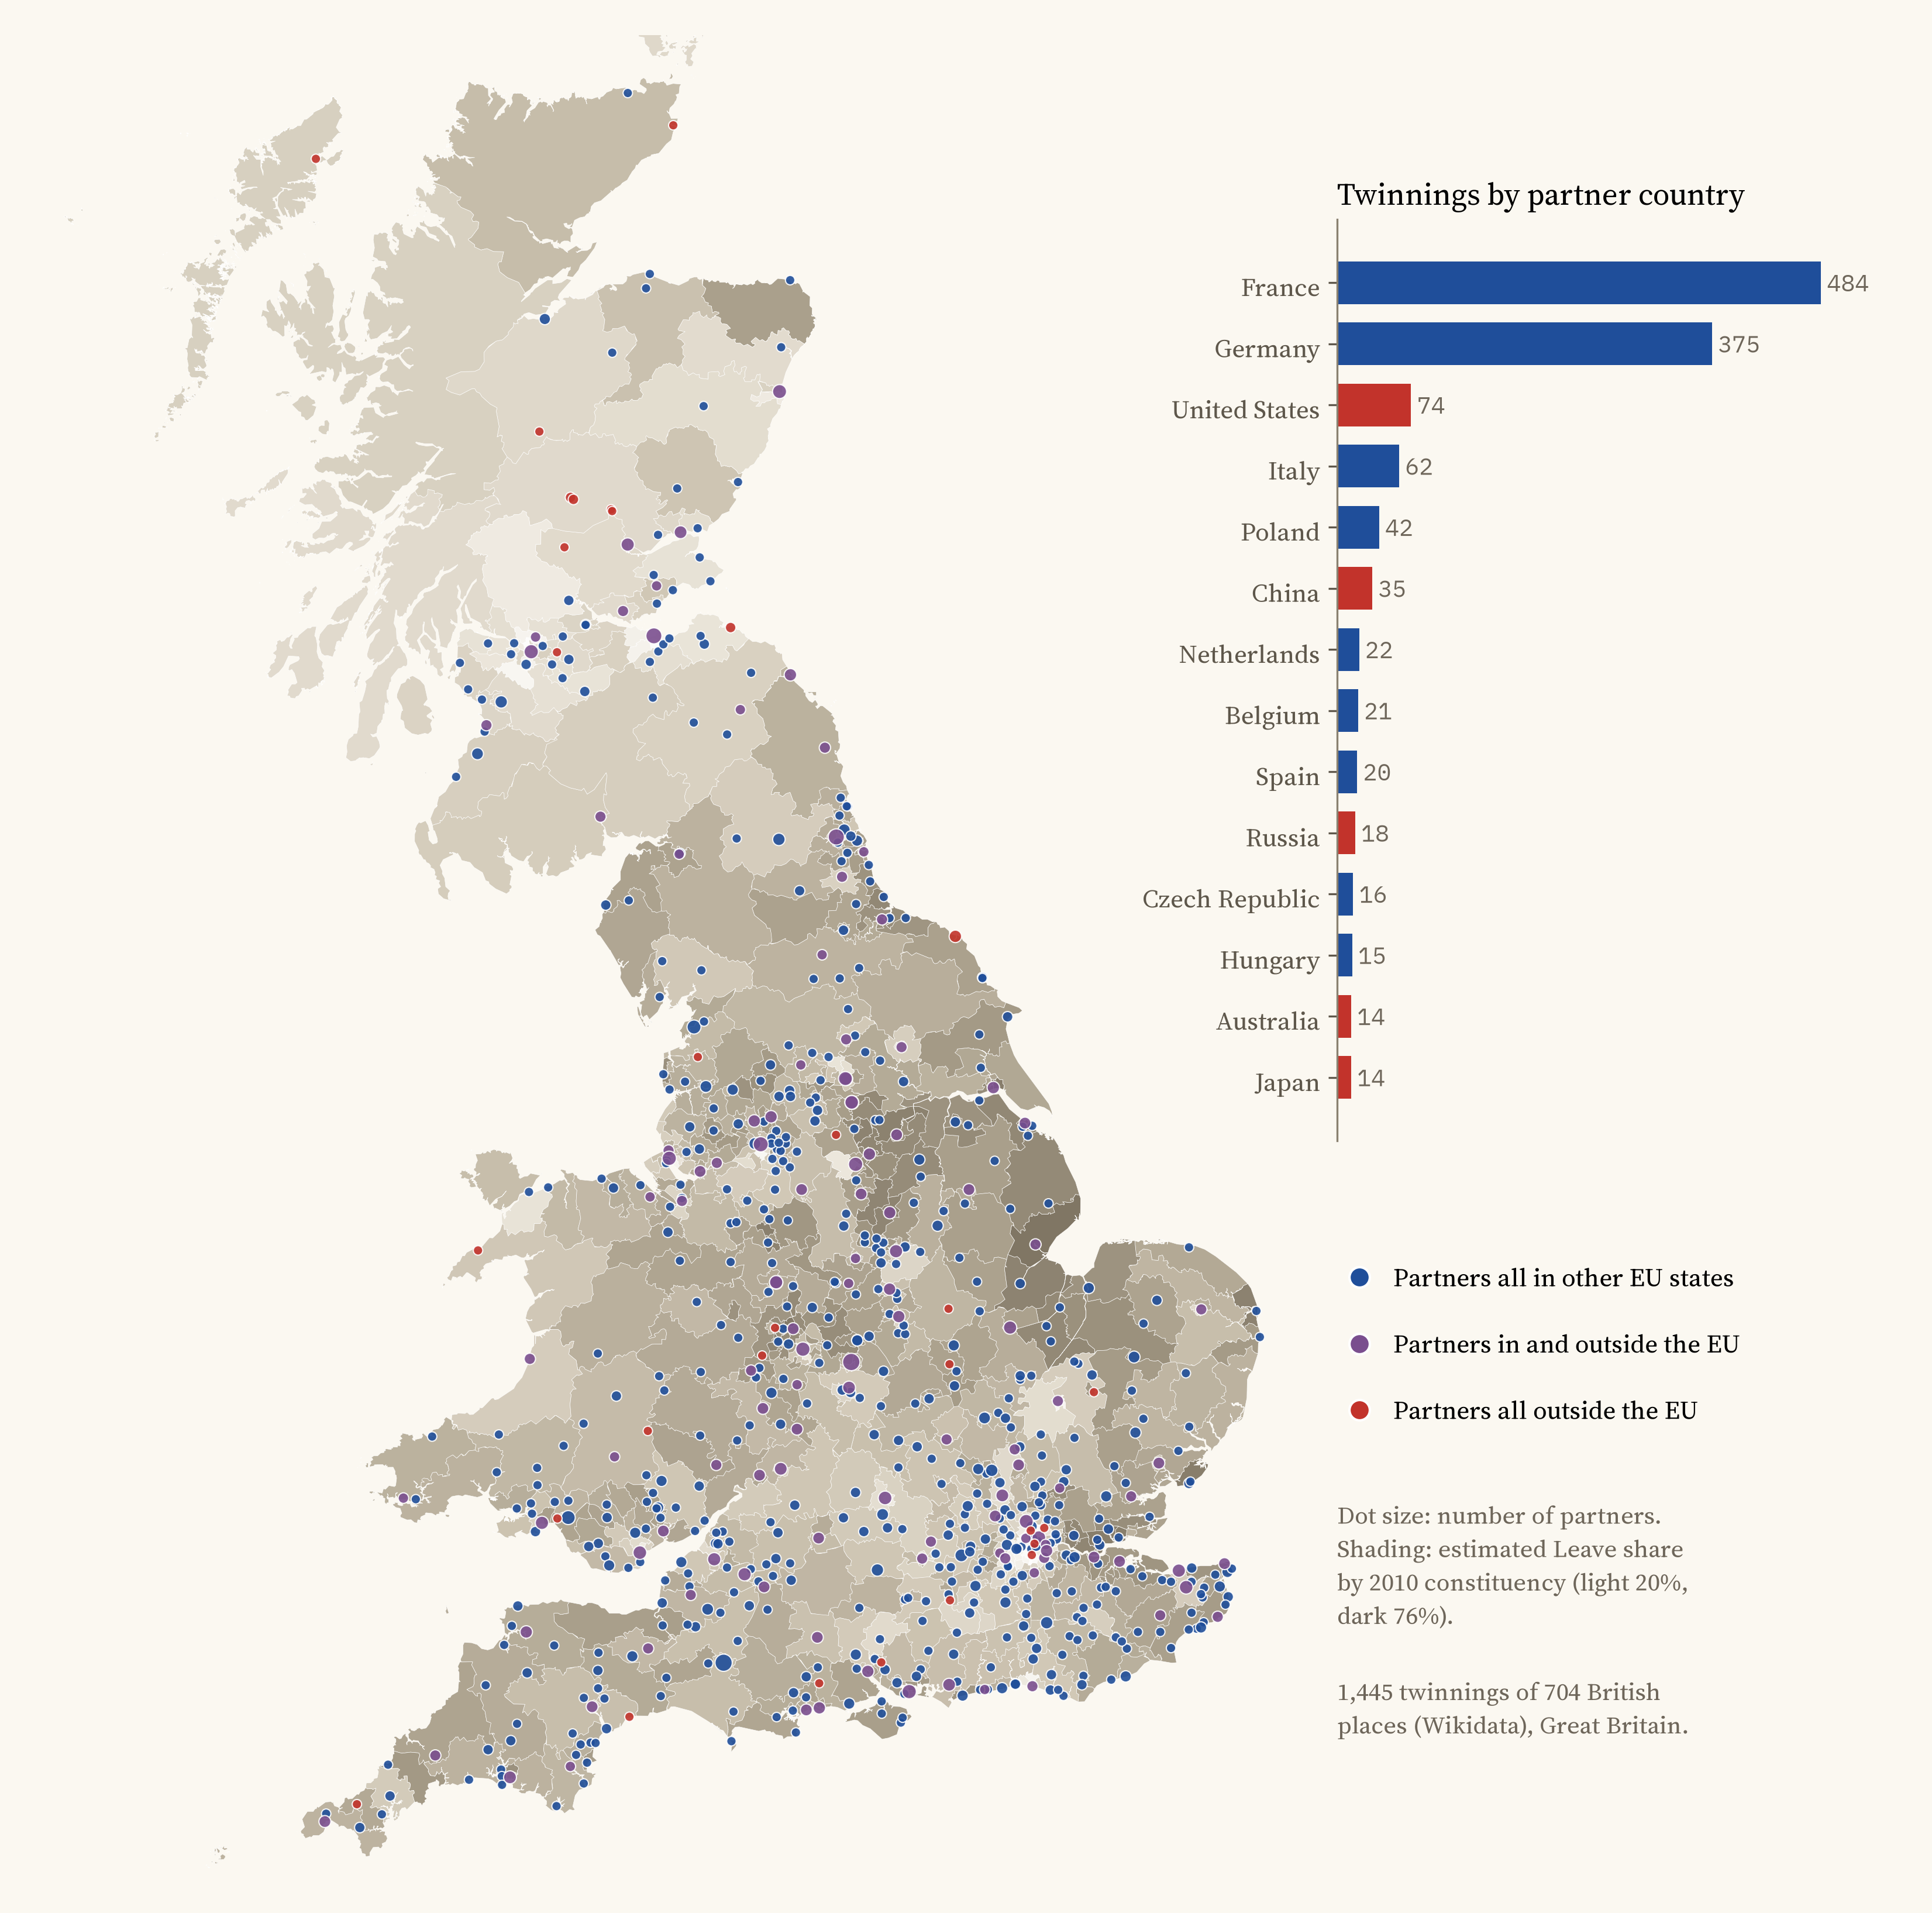
\includegraphics[width=0.98\textwidth]{f_map.png}
\caption{Twinned places in Great Britain by the kind of partner, over the estimated Leave share by 2010 constituency (grey shading). Dot size: number of partners. Bars: usable twinnings by partner country (the fourteen largest).}\label{fig:map}
\end{figure}

\subsection{Hosts and their constituencies}
A twinning in Wikidata is attached to an item, and that item may be a town, a village, a parish, a district, a city council area or a county. The distinction matters because most English and Welsh twinnings are made by district or city councils, whose areas can contain several constituencies, while many others are made by town or parish councils. I classified the 747 host items by rules fixed in the analysis plan (Table~\ref{tab:hosts}). A host is a local authority host if its name matches the name of a 2013 local authority district (after removing prefixes such as ``City of'' and ``London Borough of'' and suffixes such as ``City'') and its point lies in or within 5 km of that district. Its twinnings are assigned to every constituency with at least a third of its area in that district, and to the constituency holding the point. Other hosts (towns, villages, parishes and districts abolished before 2013) are settlement hosts, and their twinnings go to the constituency containing their point. 12 wide-area hosts (Greater London, shire and metropolitan counties, former regions and historic counties), 13 schools and 17 places outside Great Britain (in Northern Ireland, Gibraltar, Guernsey and the Cayman Islands) were excluded from the main exposure. One documented override assigns Brighton's twinnings to Brighton and Hove, whose council makes them. Two rule errors found in a check of all hosts with three or more partners, before any text was written, were corrected: Scottish council areas named ``Glasgow City'', ``Aberdeen City'' and ``Dundee City'' were not matched by the first version of the rule, and a ``Greater London'' item was treated as a settlement. The correction moved the main estimate from $-0.13$ to -0.30 points and changed no conclusion (Appendix~\ref{app:data}).

For each constituency the exposure is the number of distinct EU partners reached by its hosts and the number of distinct non-EU partners. On these rules 566 of the 632 seats (90\%) have at least one EU partner, 252 (40\%) have at least one non-EU partner, 12 have only non-EU partners and 54 have none recorded. The median seat has 2 EU partners. That most seats are exposed is a consequence of council twinning: a twinning made by Leeds City Council counts for all eight Leeds seats.

\subsection{Coverage of the source}
Wikidata records twinning unevenly. Figure~\ref{fig:coverage} shows the share of settlements with an English Wikipedia article that are themselves twinning hosts, by population. It rises from 0.4\% of places under 2,000 people and 5.9\% of those with 2,000 to 9,999, to 17\% of places of 10,000 to 49,999 and 58\% of the 246 places of 50,000 or more. Some of this gradient is real (larger places twin more), and some probably reflects the attention that editors give to larger places; user-generated sources are known to cover places very unevenly \citep{graham2014}. Many British towns that twin, often through a town council or a twinning association rather than the district, are probably missing, and some recorded twinnings are dormant. Only 26\% of EU twinnings have a start date. I could not validate the record against council lists, because no external register was available for this study; the analysis therefore treats the exposure as recorded twinning and adjusts for the two most obvious drivers of recording, settlement size and the number of documented settlements in a seat. Measurement error of this kind, if unrelated to the vote once these controls are held fixed, biases the estimates towards zero; I return to this in Section~\ref{sec:disc}.

\begin{figure}[tbp]\centering
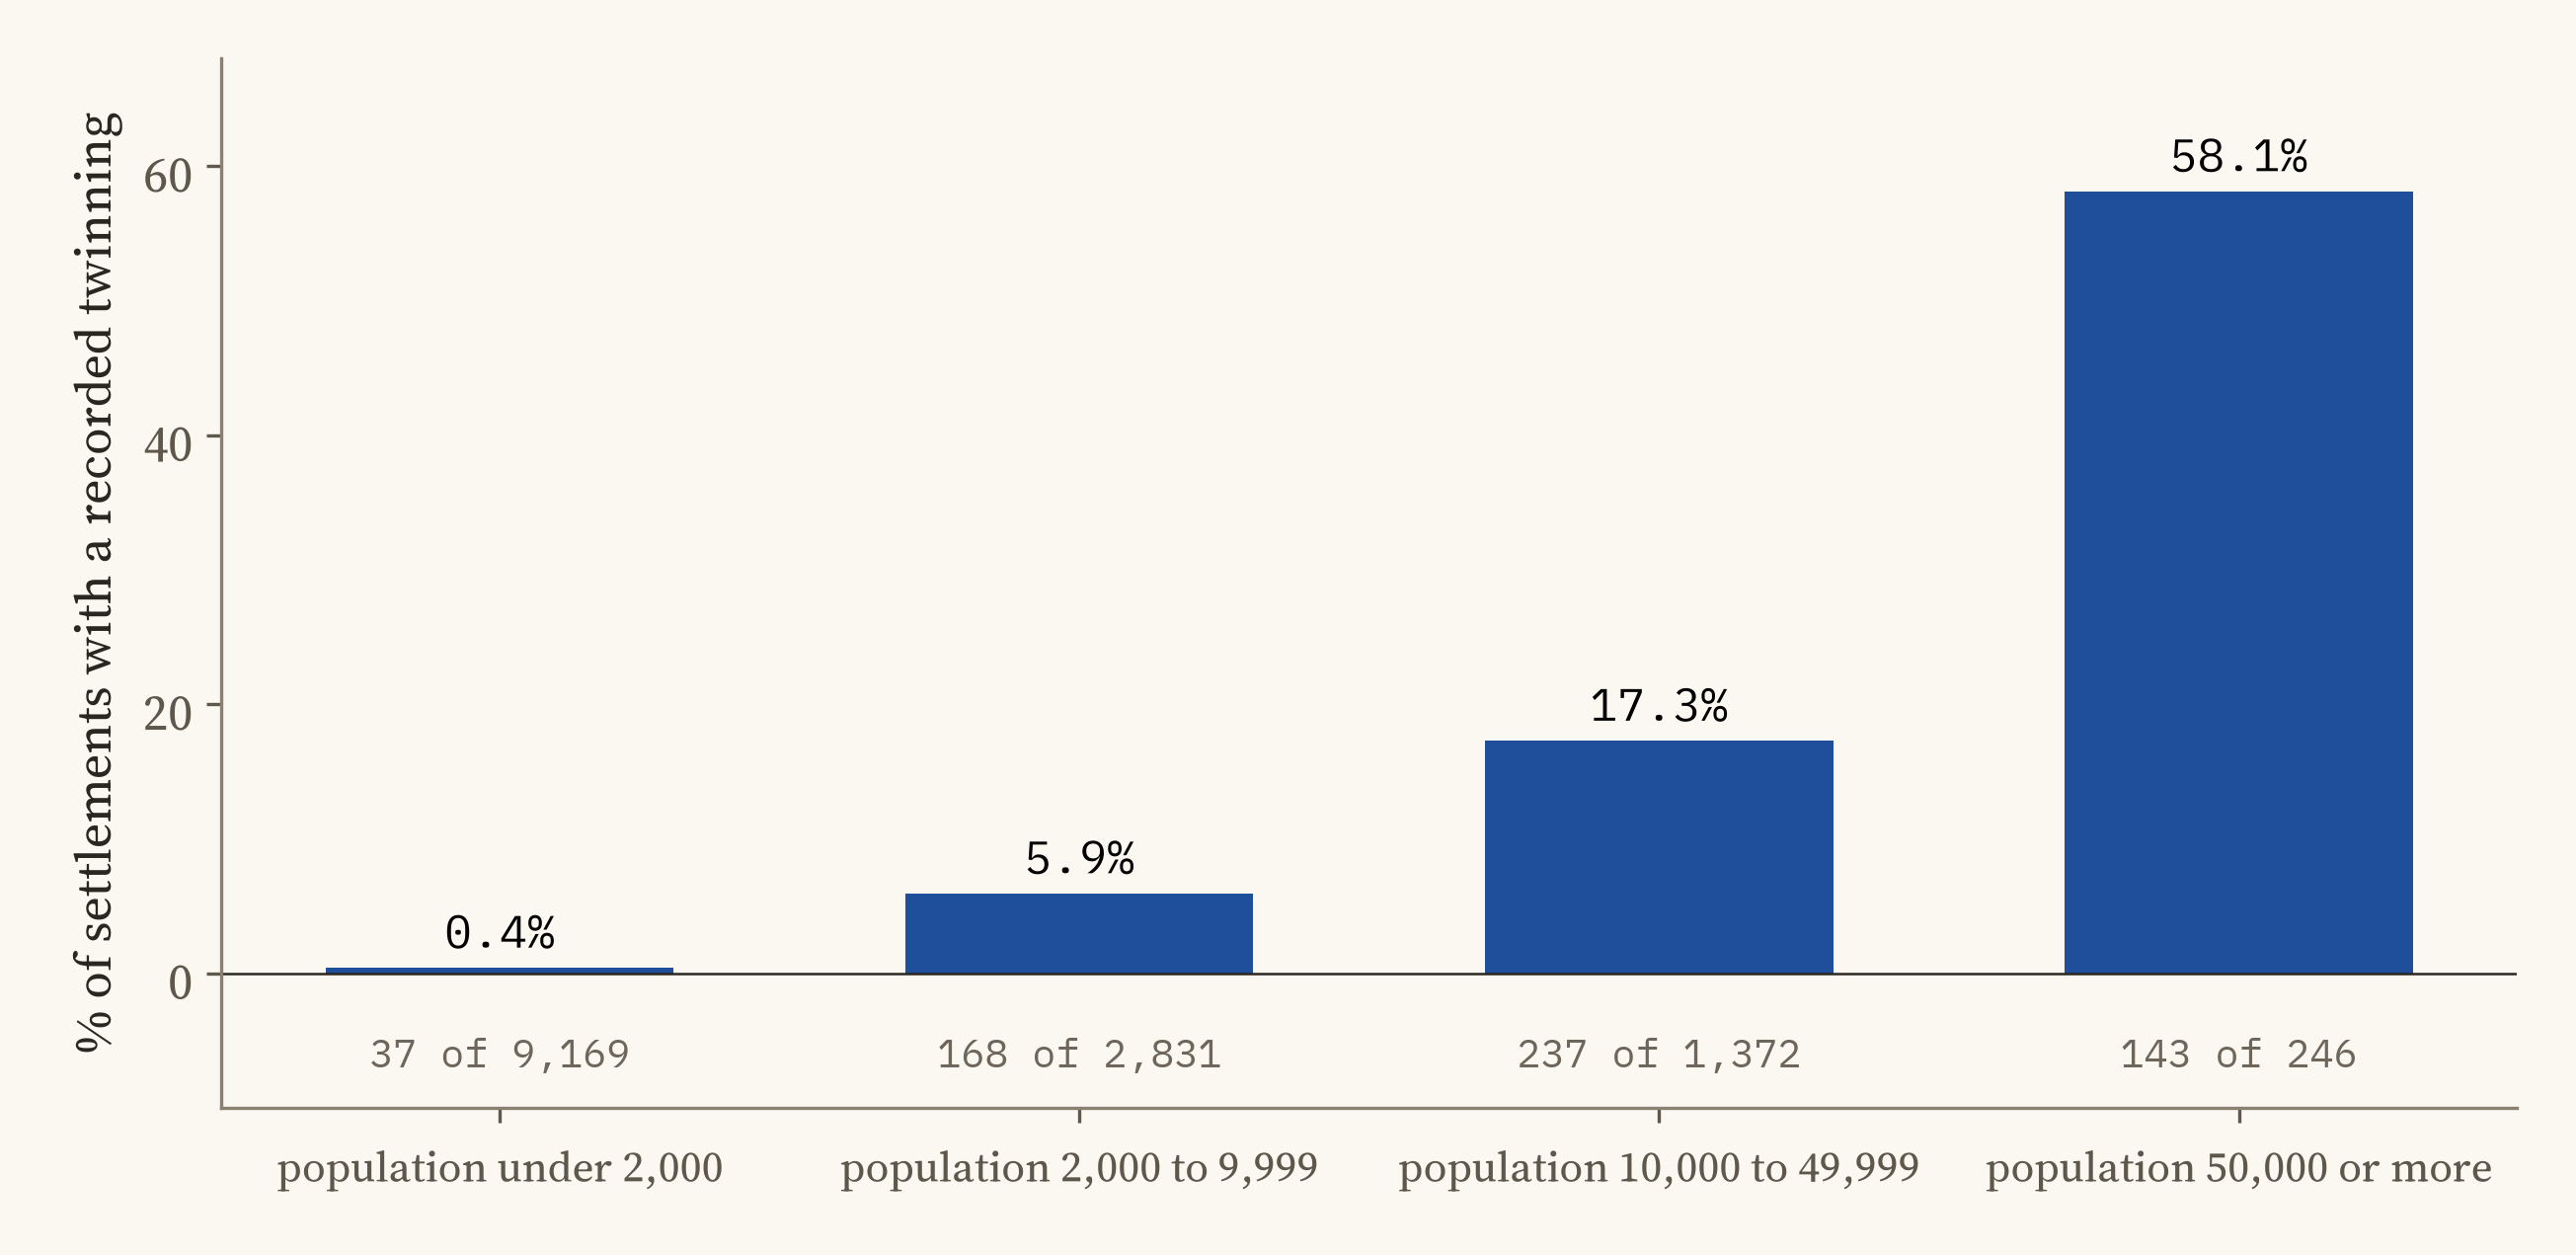
\includegraphics[width=0.85\textwidth]{f_coverage.png}
\caption{Share of settlements with an English Wikipedia article that are recorded as twinning hosts in Wikidata, by population band (population as stated in Wikidata). Below each bar: hosts of all settlements in the band.}\label{fig:coverage}
\end{figure}

\subsection{Outcome and controls}
The outcome is the estimated Leave share of each 2010 constituency in Great Britain \citep{hanretty2017}, as compiled in the parlitools package \citep{parlitools}, in percentage points (mean 52.1, standard deviation 11.4). The controls are those of the aggregate Leave literature, from the 2011 census by constituency: the share of residents aged 65 or over, the share with a degree-level qualification, the share with no qualifications, the share of working-age residents in routine and semi-routine occupations, the White British share, the share born outside the United Kingdom, and log population density; with fixed effects for the nine English regions, Wales and Scotland. Because twinning is recorded more often for larger and better documented places, the plan added three controls for documentation and settlement structure: the log of one plus the number of settlements in the seat with an English Wikipedia article, the log of one plus the population of the largest such settlement, and an indicator for county (as opposed to borough) constituencies. Table~\ref{tab:desc} compares seats with and without an EU twin on these variables.

The region fixed effects matter for this question because both twinning and the vote have strong regional patterns. Scotland voted Remain in 57 of its 59 seats and has its own local government geography, with large council areas whose twinnings spread over many seats; London voted Remain in 57 of its 73 seats and its boroughs twin as councils; and the English regions differ in the age of their towns and in how much their councils have recorded. Comparing seats within regions removes these contrasts. The census controls follow the established aggregate models \citep{becker2017,goodwin2016}; they are measured five years before the referendum, which is close enough for slowly changing population characteristics. The documentation controls are specific to this study: they are meant to absorb the tendency of larger and better documented places both to have recorded twinnings and to have particular electorates.

\section{Research design}\label{sec:design}
\subsection{Analysis plan}
The plan (NOTES.md in the replication files, section 0) was written after reading the twinning data and the lists of census and Leave variables, and before any twinning count had been joined to a Leave share. It specified three hypotheses. H1: seats with at least one EU twinning have a lower Leave share than otherwise similar seats. H2: the EU twinning gap is more negative than the gap for non-EU twinning in a model with both, and among twinned seats a higher EU share of partners goes with lower Leave. H3 (secondary): twinnings formed before British accession in 1973 go with a larger gap than later ones. It stated in advance that H1 fails if the 95\% interval includes zero and the point estimate is smaller in size than one point, and that a significant EU estimate matched by the non-EU placebo would indicate that the association concerns the kind of place that twins rather than Europe.

\subsection{Main specification}
The main model is an ordinary least squares regression of the Leave share on an indicator for at least one EU partner and the controls above:
\begin{equation}
\text{Leave}_{i} = \beta\,\text{EU}_{i} + \mathbf{x}_{i}'\gamma + \alpha_{r(i)} + \varepsilon_{i},
\end{equation}
where $i$ indexes constituencies, $\mathbf{x}_i$ holds the census and documentation controls and $\alpha_r$ are region fixed effects. Standard errors are clustered by the local authority that holds most of each seat's area (356 clusters), because council-level twinnings make seats in one council area share their exposure \citep{cameron2015}. I report $\beta$ in percentage points of Leave with a 95\% interval based on the $t$ distribution with one fewer degree of freedom than there are clusters, and an equivalence test with a smallest effect of interest of one point \citep{lakens2017}.

The binary exposure was chosen as the main measure because it is least sensitive to the uneven recording of partners: a seat either has a recorded European twin or it does not. Counts and rates per head are planned alternatives.

\subsection{Europe or twinning}
The H2 tests add an indicator for at least one non-EU partner. The planned placebo is the model with the non-EU indicator alone; the joint model tests whether the EU and non-EU coefficients differ. Among seats with any twinning, a second test regresses Leave on the EU share of partners, controlling for the log of the number of partners.

\subsection{Robustness and falsification}
The planned checks vary the exposure (log count of EU partners; log EU partners per 100,000 residents; assignment to the point's seat only, without spreading council twinnings; twinnings begun after the referendum removed; EU-15 partners only; French and German partners only; wide-area hosts added), the sample and outcome (seats with counted ward-level figures; the model-only estimate of \citealt{hanretty2017}; England only; without London; without the 1\% of seats with the largest Cook's distance) and the specification (no documentation controls; local authority fixed effects, which compare seats within one council area and so rely only on town-level twinnings; the share born in Ireland or other EU states added). Spatial dependence is addressed with \citet{conley1999} standard errors at 50 and 100 km. Every region is left out in turn. A nearest-neighbour match within region on the standardised controls, with a regression bias correction \citep{abadie2006}, compares EU-twinned seats with seats without an EU twin. Randomisation inference shuffles the EU indicator within regions 2,000 times. Sensitivity to unobserved confounding is gauged with the coefficient-stability approach of \citet{oster2019}.

\subsection{Threats to inference}
Three threats deserve emphasis. First, selection: councils choose to twin, and places that twin may be larger, older and more civic, which the controls only partly capture. The non-EU placebo addresses the part of selection that concerns twinning in general. Second, measurement: recorded twinning is an incomplete and noisy measure of actual links, and a twinning link says nothing about how many residents took part. Both make an effect harder to detect; the minimum detectable effect is reported. Third, the outcome is an estimate for most seats, with modelling error correlated with census variables. The checks on counted results and the model-only estimate address this.

\section{Results}\label{sec:results}
\subsection{Descriptive patterns}
Seats with an EU twin and seats without look alike on the main predictors of the Leave vote (Table~\ref{tab:desc}). Seats with an EU twin have a slightly lower degree share (26.6\% against 27.9\%), a slightly lower share aged 65 or over (16.7\% against 17.5\%) and higher density. Their mean Leave share is 52.1\%, against 51.5\% for the 66 seats without an EU twin. Figure~\ref{fig:bins} shows the raw Leave share and degree share by the number of EU partners: there is no gradient in either. Seats with six or more EU partners voted Leave at 50.6\%, much like seats with none (51.5\%).

\begin{figure}[tbp]\centering
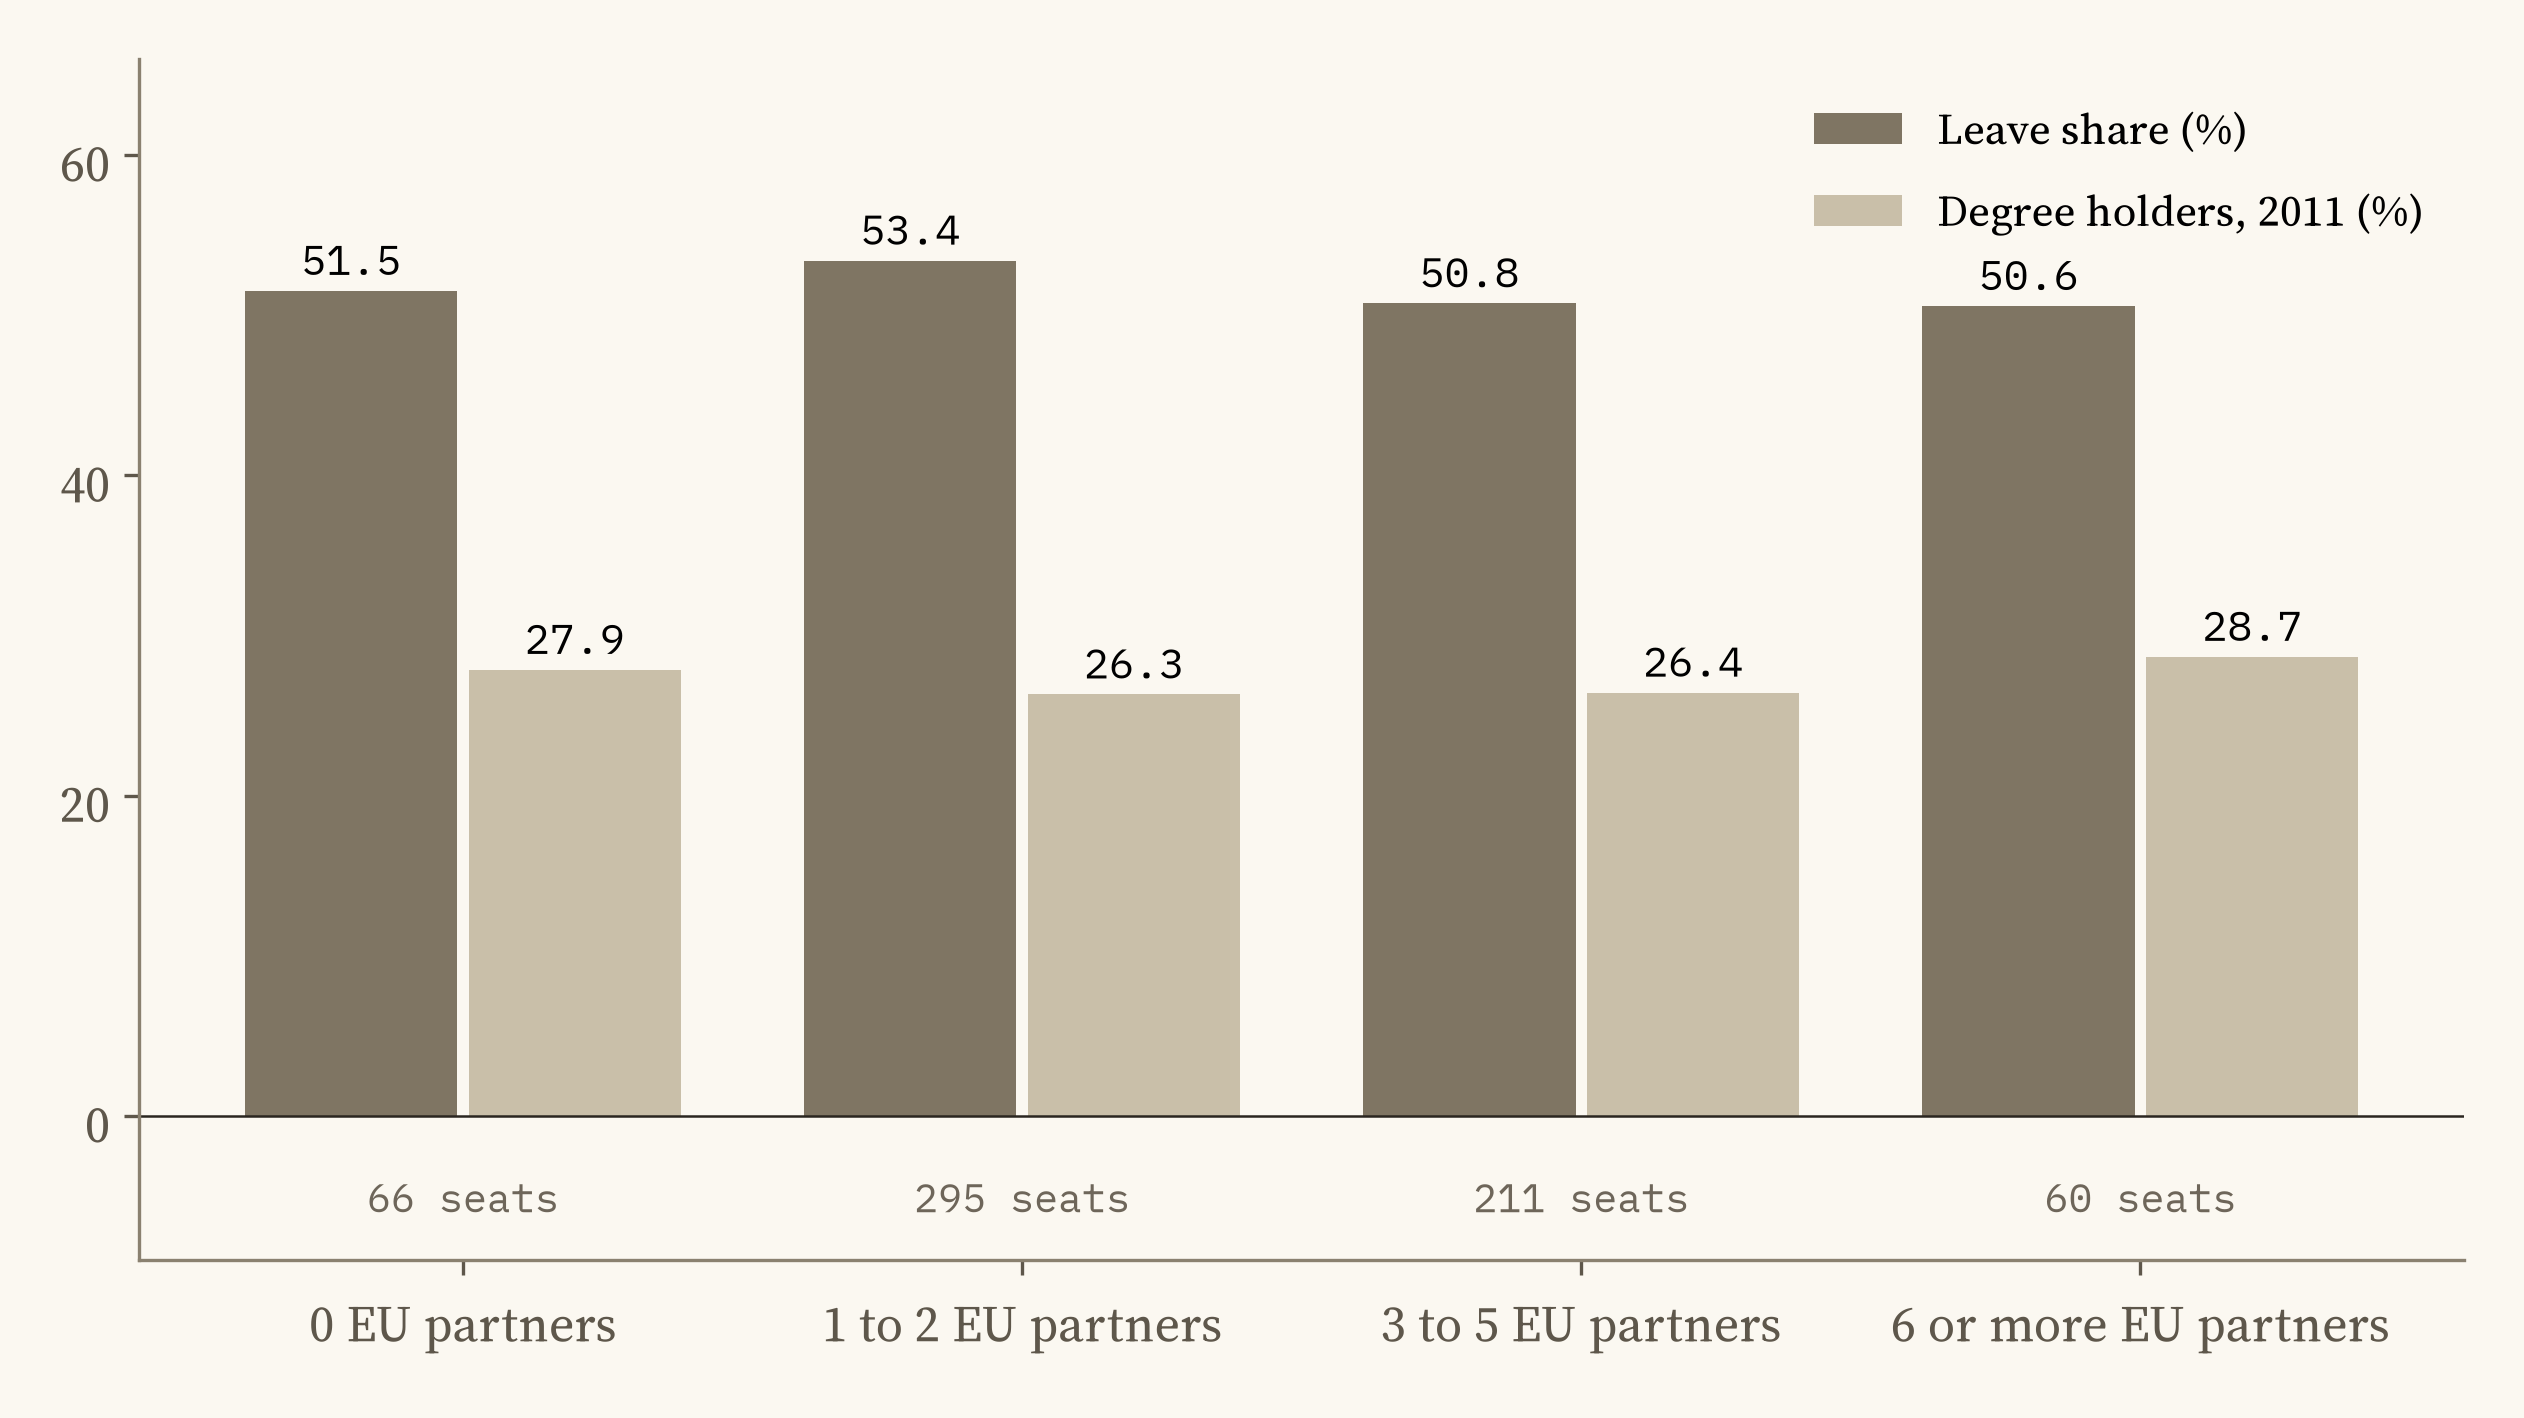
\includegraphics[width=0.85\textwidth]{f_bins.png}
\caption{Mean estimated Leave share and mean degree share (2011) by the number of EU partners of the seat. Raw means, no controls.}\label{fig:bins}
\end{figure}

\subsection{Main result}
Table~\ref{tab:ladder} reports the model ladder. The raw difference is 0.60 points (95\% CI -3.39 to 4.59): EU-twinned seats voted, if anything, slightly more Leave. Region fixed effects reduce it to 0.12; adding the census variables gives -0.31; and the planned main model, which adds the documentation controls, gives -0.30 points (95\% CI -1.40 to 0.80; $p$ = 0.59; N = 632; $R^2$ = 0.88). By the criterion fixed in advance, H1 fails: the interval includes zero and the point estimate is smaller in size than one point.

The null is reasonably precise. The interval excludes a Remain association larger than 1.4 points, about 12\% of a standard deviation of the Leave share across seats. The minimum effect the design could detect with 80\% power at the 5\% level is 1.6 points. An equivalence test against a smallest effect of interest of one point is not passed ($p$ = 0.11; 90\% CI -1.23 to 0.62), so the data cannot rule out an association of about one point. They do rule out the kind of difference that would make twinning a meaningful part of the referendum's geography.

\subsection{Europe or twinning}
The planned placebo gives a different picture (Table~\ref{tab:ladder}, lower panel; Figure~\ref{fig:forest}). Seats with at least one non-EU partner had a Leave share 1.37 points lower than otherwise similar seats (95\% CI -2.26 to -0.48; $p$ = 0.003). In the joint model the non-EU coefficient is -1.36 and the EU coefficient -0.03. The planned difference test (EU minus non-EU) is 1.34 (95\% CI -0.23 to 2.91; $p$ = 0.095): the point estimate runs against H2, though the interval is wide. Among the 578 seats with any twinning, a ten-point higher EU share of partners is associated with a Leave share 0.12 points different (95\% CI -0.10 to 0.34). With count measures of both kinds of twinning in one model, the coefficient on log EU partners is -0.27 (95\% CI -0.96 to 0.43) and on log non-EU partners -1.08 (-2.00 to -0.17). H2 fails: there is no sign that European partners, rather than partners in general, mark out more Remain places.

The non-EU partners are mostly in the United States, China, Russia, Ukraine and Japan: 119 seats have an American partner and 89 a Chinese one. These are the twinnings of cities and large towns: the median largest settlement in seats with a non-EU partner has 38,448 people, against 30,984 in other seats. The controls include the size of the largest settlement, but a single number cannot capture what makes a place a regional centre with links across the world.

\begin{figure}[tbp]\centering
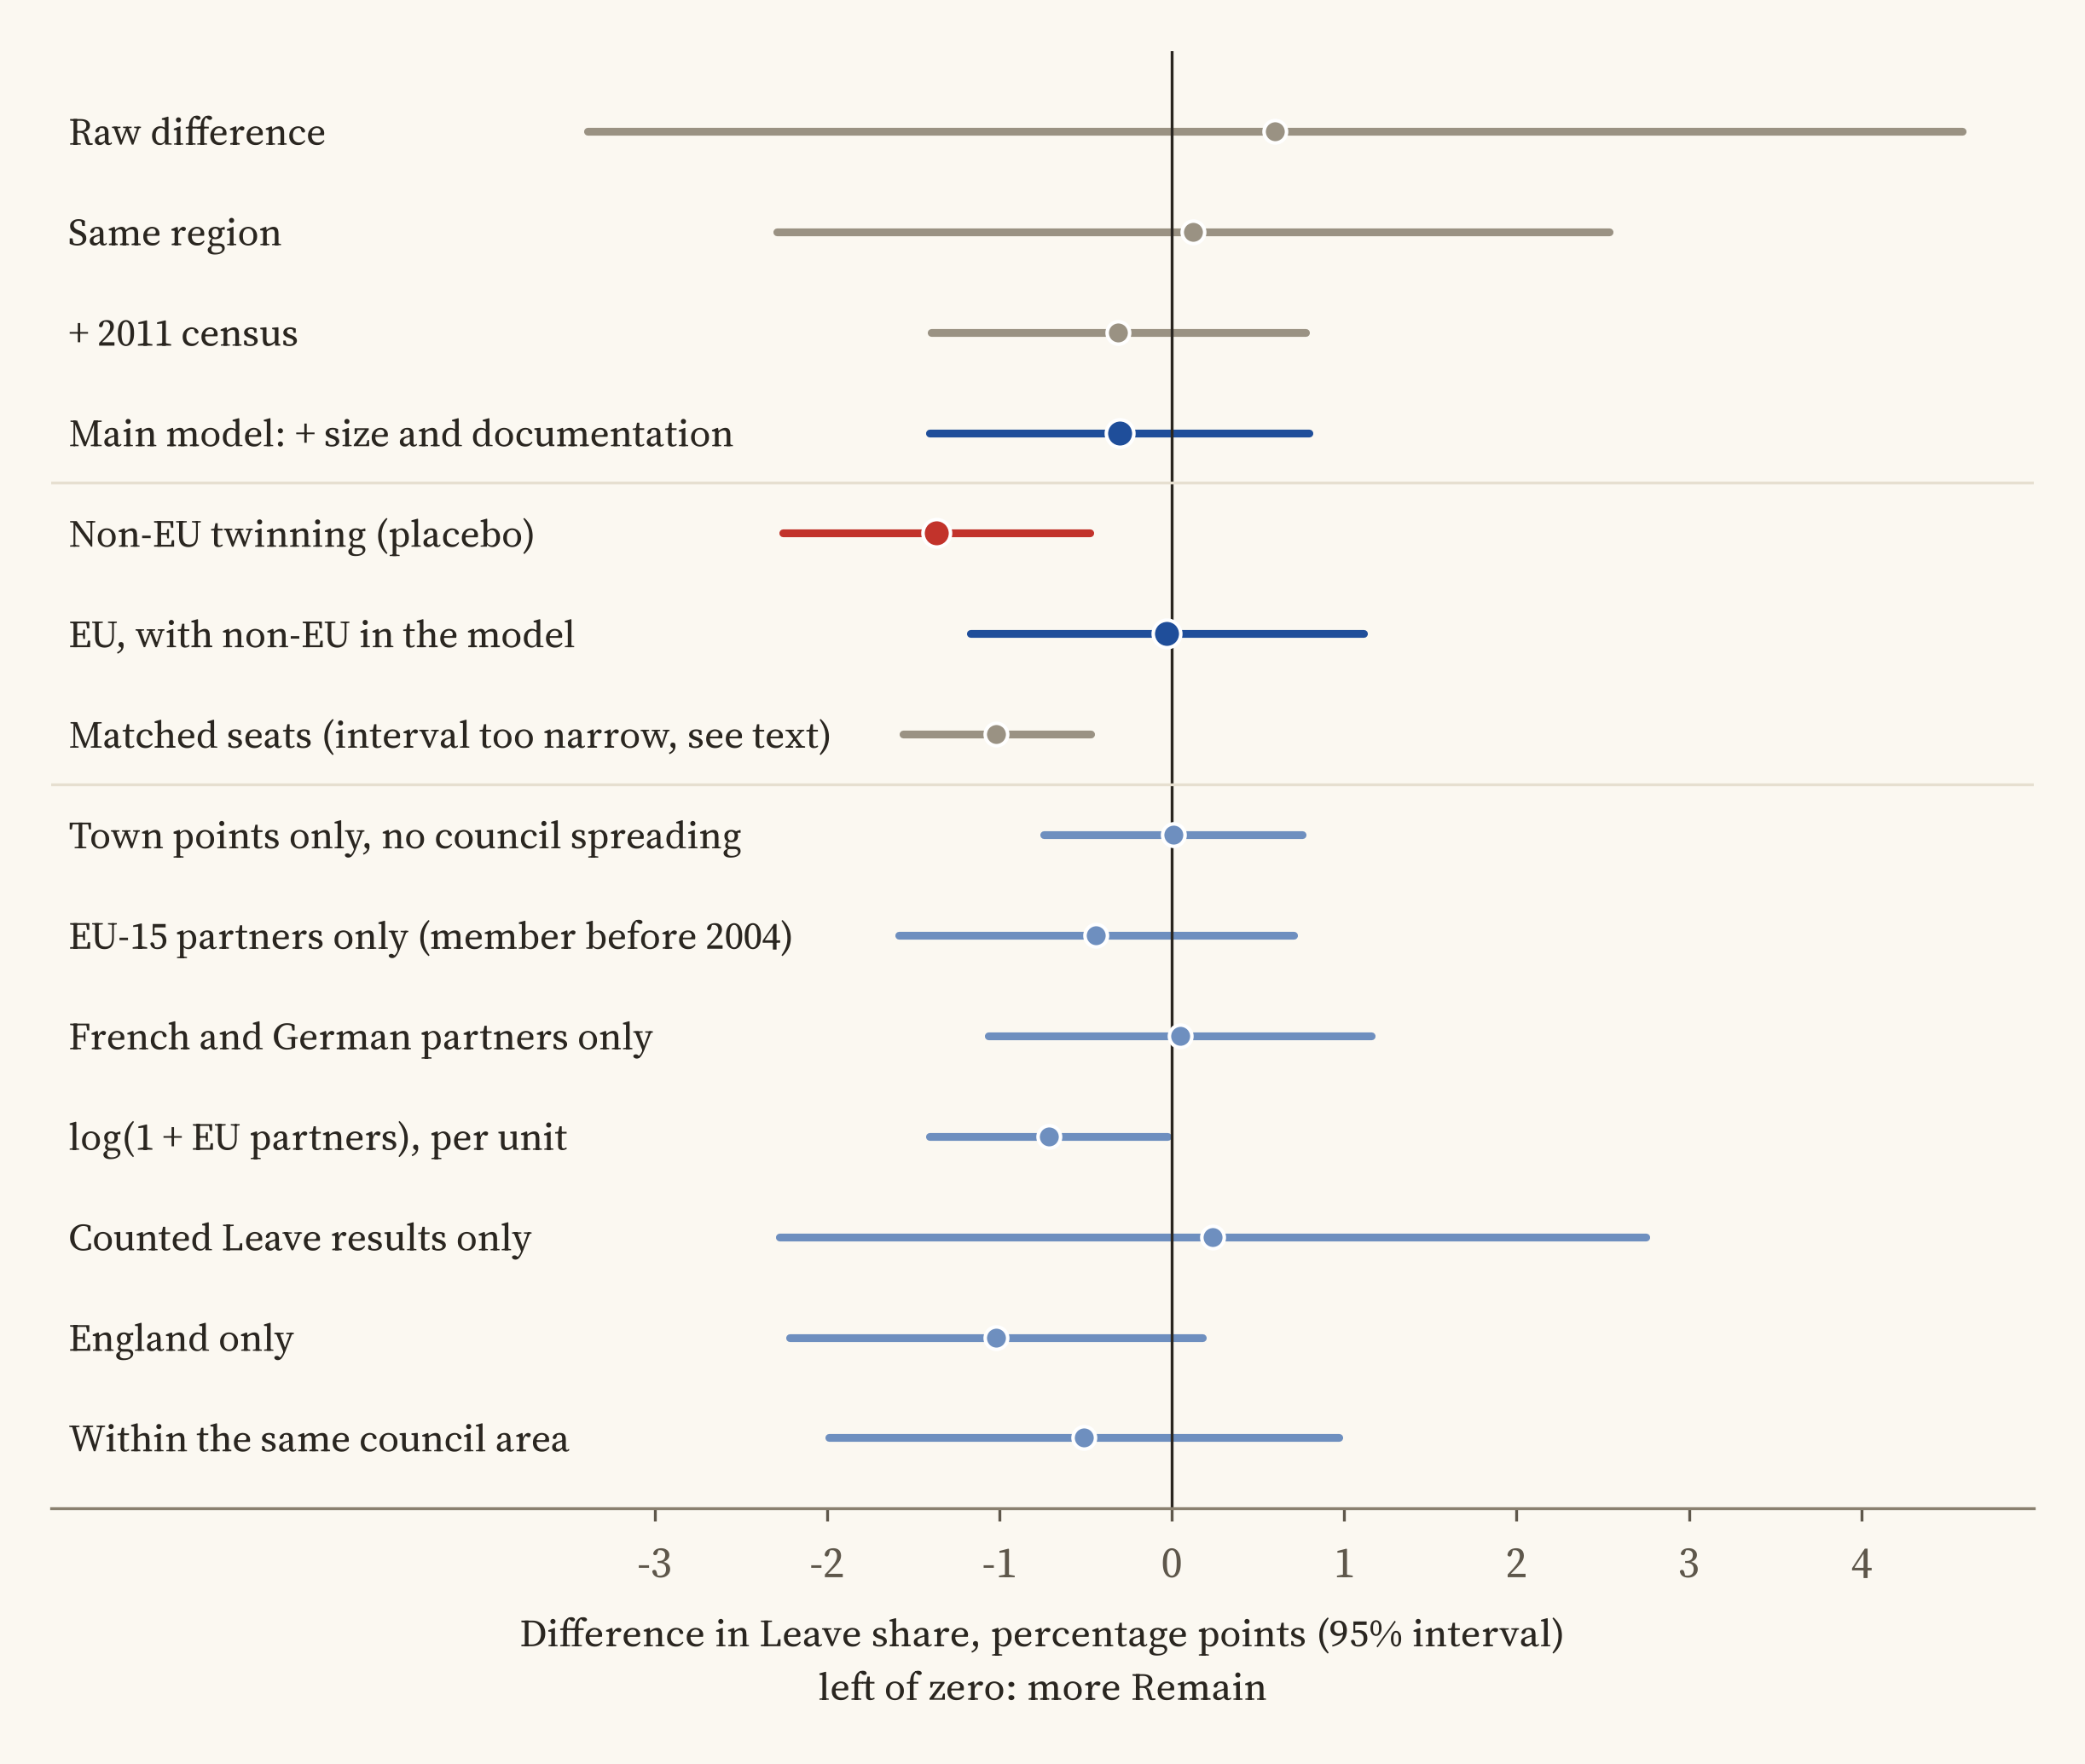
\includegraphics[width=0.92\textwidth]{f_forest.png}
\caption{Estimates with 95\% intervals, in points of Leave. Top: the model ladder for an EU twin. Middle: the non-EU placebo, the EU coefficient with the non-EU indicator in the model, and the matched comparison (whose bootstrap interval ignores matching uncertainty). Bottom: planned robustness checks. The log count row is per unit of log(1 + EU partners).}\label{fig:forest}
\end{figure}

\subsection{Timing}
Only 298 of the 1,148 EU twinnings (26\%) have a start date. Of these, 109 began before 1973 and 189 in or after 1973 (Figure~\ref{fig:timing}); the dated links peak in the 1990s, the decade after the changes in Eastern Europe that \citet{falkenhain2012} identify as a turning point for twinning. 5 EU twinnings are recorded as beginning after the referendum. Among the 283 seats with at least one dated EU twinning, seats whose first dated EU twin is older than 1973 had a Leave share -0.29 points different from seats whose first dated EU twin came later (95\% CI -1.94 to 1.37). H3 receives no support, although with three quarters of the dates missing the test is weak. Two EU twinnings are recorded as ending after the referendum (Edinburgh with Krak\'ow and Braintree with Pierrefitte-sur-Seine), too few to say anything about whether the vote affected twinning.

\begin{figure}[tbp]\centering
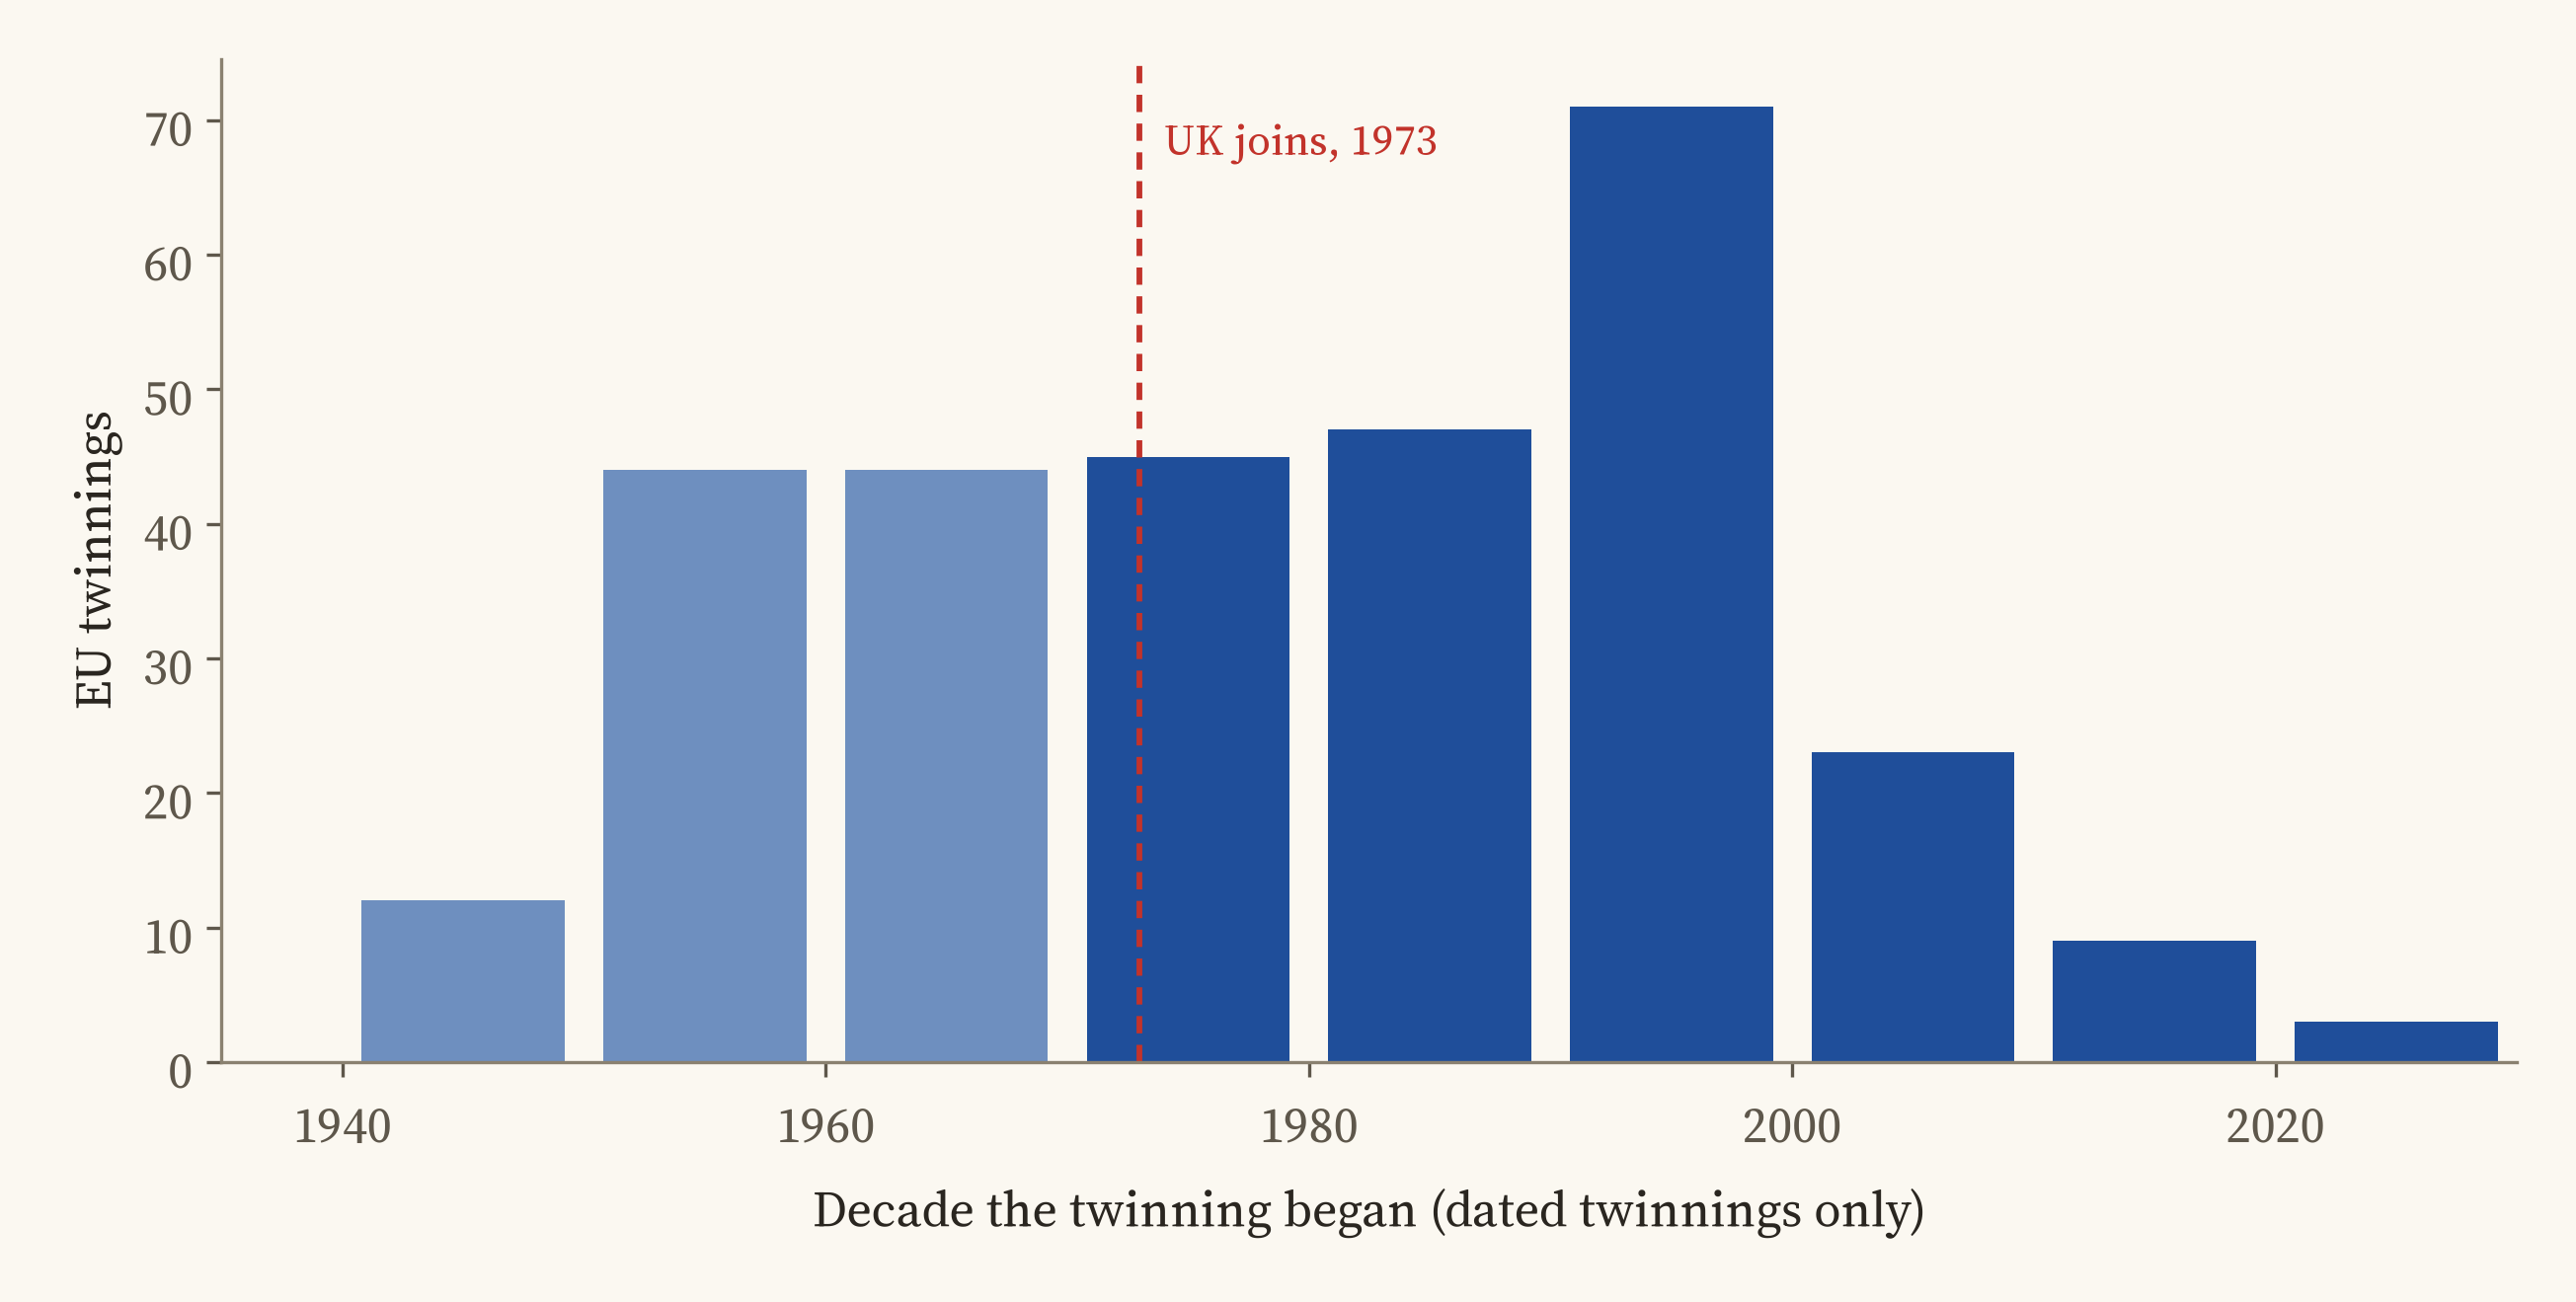
\includegraphics[width=0.85\textwidth]{f_timing.png}
\caption{Dated EU twinnings by the decade they began. Lighter bars: decades before British accession. Only 26\% of EU twinnings have a start date in Wikidata.}\label{fig:timing}
\end{figure}

\section{Robustness}\label{sec:robust}
\subsection{Planned checks}
Table~\ref{tab:robust} reports the planned checks. Assigning twinnings only to the seat holding the host's point, without spreading council twinnings, gives 0.01 (95\% CI -0.74 to 0.76). Restricting partners to the EU-15 gives -0.44, and to France and Germany, the oldest and most numerous twinning partners, 0.05. Adding the wide-area hosts gives -0.11; removing twinnings begun after the referendum changes nothing, because no seat's exposure depends on them. On the 128 seats with counted ward-level results the estimate is 0.24 (95\% CI -2.28 to 2.75), and with the model-only estimate as outcome -0.48. England alone gives -1.02 (-2.21 to 0.18); without London, -0.30. Within local authorities, where only the 21 councils whose seats differ in exposure contribute, the estimate is -0.51 (-1.99 to 0.97).

Two of the fifteen checks are significant at the 5\% level, both using counts rather than the indicator: one more unit of log(1 + EU partners) is associated with -0.71 points (95\% CI -1.40 to -0.02), and the log rate per 100,000 residents with -0.67 (-1.34 to 0.00). These are small: one unit of log(1 + partners) is roughly the step from one EU partner to four. More importantly, once the log count of non-EU partners is in the model, the EU count is -0.27 and not significant (Section~\ref{sec:results}). The count measures pick up places with many partners of every kind.

Leaving out each region in turn gives estimates from -0.77 to 0.17, none significant (Table~\ref{tab:loro}). Conley standard errors give 95\% intervals of -1.34 to 0.73 at 50 km and -1.54 to 0.94 at 100 km. Randomisation inference, shuffling the indicator within regions, finds an estimate at least as large in 1,175 of 2,000 draws ($p$ = 0.59).

\subsection{Matching and sensitivity}
The matched comparison is the strongest planned evidence against the null. Matching each of the 566 EU-twinned seats to the most similar seat without an EU twin in the same region (with replacement; 58 distinct control seats used) reduces the largest standardised difference in the controls from 0.41 to 0.27, and the bias-corrected difference is -1.02 points (bootstrap 95\% interval -1.56 to -0.47). Two features make this weaker than it looks. The naive bootstrap understates the uncertainty of nearest-neighbour matching with replacement, because it ignores the reuse of a small pool of 66 controls, many of them several times; and the result is not matched by the regression, randomisation or within-council estimates, which use all seats. An exploratory bootstrap added at review, which resamples seats within regions and repeats the matching in each of 500 draws, gives a 95\% interval of -3.04 to 0.63, which includes zero; and matching that also requires the control seat to share the treated seat's non-EU twinning status (474 matched seats) gives -0.32 (naive interval -0.84 to 0.22). I read the planned matched estimate as consistent with a Remain association of up to about one point, which the main interval also allows, and not as evidence of one.

Coefficient stability is uninformative here in the usual sense, because the controls move the estimate across zero: the Oster bias-adjusted coefficient for equal selection on observed and unobserved variables is -0.43. The movement from the raw to the controlled estimate is itself the main lesson: what little raw difference there is between EU-twinned and other seats comes from where they are and who lives there.

\subsection{Exploratory analyses}
Two analyses were added after the planned analysis and are exploratory. First, removing twinnings that Wikidata records as having ended before the referendum (the Neath Port Talbot links, among others) leaves the estimate unchanged (-0.30). Second, because the non-EU placebo was significant, I subjected it to the same checks as the main estimate (Table~\ref{tab:noneu}). The non-EU association survives leaving out any region (11 of 11 estimates significant), England alone (-1.78), the omission of London and the model-only outcome. It does not survive local authority fixed effects (-0.74, 95\% CI -2.59 to 1.12) or the restriction to seats with counted results (0.58, -1.79 to 2.95). Most non-EU twinnings are made by city and district councils, so within-council comparisons remove most of the variation; the association is therefore a contrast between council areas, and council areas with links to the United States or China differ in many ways that seat-level controls do not capture.

Two further exploratory checks were added at an independent review of the analysis (as were the two matching checks in the previous subsection). First, clustering by local authority treats seats in different councils as independent, although a council's twinnings are spread to every seat with a third of its area in that council. Clustering instead on groups of seats linked by any shared council host (324 clusters) gives a 95\% interval of -1.42 to 0.81 for the EU indicator, and leaves the non-EU coefficient significant (-2.26 to -0.47). Second, because Wikidata's coverage is best for large places, I repeated the main model on the 226 seats whose largest documented settlement has 50,000 people or more: the EU estimate is 0.30 (95\% CI -1.67 to 2.26), but only 19 of these seats lack an EU twin, so the test is weak; the non-EU coefficient there is -1.26 (95\% CI -2.64 to 0.12).

\section{Discussion}\label{sec:disc}
\subsection{What the results say}
The hypothesis that European twinning made places more pro-European is not supported at the level of constituencies. Seats with a recorded EU twin voted like comparable seats without one; the estimate is null in all but two of the planned checks, and those two (count measures) lose their association once non-EU partners are counted. Where there is any association between twinning and the referendum vote, it is with twinning outside the EU, and that association looks like a property of the kind of place, larger and better connected council areas, rather than of contact with Europe.

There are good reasons to expect a null even if twinning matters for those who take part. Individual-level research finds that transnational experience is concentrated among the young and educated \citep{kuhn2015,fligstein2008}, and organised exchanges reach selected participants \citep{sigalas2010,mitchell2015}. A twinning association might involve a few hundred people in a constituency of seventy thousand electors. Even a large effect on participants would move the constituency share by a fraction of a point, below what this design can detect. The null therefore bounds the place-level footprint of twinning, not its effect on individuals.

The results also speak to how twinning had changed by 2016. Case studies describe declining activity, managerial forms and the pressure of local government austerity \citep{falkenhain2012,langenohl2023,warwick2024}. Wikidata records links, not activity; many links in the data may have been dormant for years. The British pattern of twinning that \citet{clarke2010} describes, civic and cultural exchange with Western Europe, may by 2016 have been more a civic tradition than a live channel of contact.


\subsection{Implications for contact and transactionalist theory}
The transactionalist argument has two versions. In the strong version, cross-border interaction spreads through societies and gradually builds a shared identity, so that places with more contact should, over time, become more European as a whole \citep{deutsch1957}. In the weak version, interaction affects those who take part, who are a selected and small part of the population \citep{fligstein2008,kuhn2011,kuhn2015}. The results here are consistent with the weak version and give no support to the strong one at the scale of the town. A twinning link sustained over decades did not leave a detectable European imprint on the vote of the constituency around it, even though such links were among the most visible and enduring forms of local European engagement in Britain.

This does not mean that contact has no political effect. The design cannot see individuals, and a place-level null is compatible with sizeable effects on the few people who participate. It does suggest that policies that rely on organised exchange to build broad public support for European integration should not expect place-level returns, at least not from the formal existence of a link. It also suggests a caution for research that uses the presence of institutions, such as twinning links, as measures of local cosmopolitanism: the non-EU association found here is the kind of pattern that such a measure would pick up, and it does not survive comparison within council areas.

A second implication concerns the interpretation of the Leave vote's geography. Explanations of the vote have stressed age, education and economic trajectories \citep{becker2017,jennings2016}, and the controls in this study absorb most of the raw differences between places. Once these are held fixed, a long-standing local institution with explicit European content explains essentially nothing more. This is consistent with accounts in which the referendum divided Britain more by who lives in places than by what those places had done \citep{hobolt2016,johnston2018}, although a single institution is a narrow test of that broader claim.

\subsection{Limitations}
Several limitations qualify these conclusions. The exposure is recorded twinning in a collaborative database, with uneven coverage by place size (Figure~\ref{fig:coverage}) and few dates; I could not validate it against council lists. If recording errors are unrelated to the vote once size and documentation are held fixed, they bias the estimates towards zero; if the places whose twinnings are recorded differ in unmeasured ways from those whose twinnings are not, the bias could go either way. The binary exposure is robust to missing partners in seats with several, but not to seats whose only twin is missing. The rules that assign council twinnings to seats are reasonable but not unique; the point-only check shows that the conclusion does not depend on them.

The design is cross-sectional. Twinning is not assigned at random, and the controls, though standard, are measured in 2011 and at the constituency level. The outcome is an estimate for most seats, and the counted-results sample is small (128 seats) and urban. Constituencies are large and mix towns with and without twins; a town-level design would need town-level results, which do not exist for the referendum. Finally, the study covers Great Britain; Northern Ireland, with its own party system and boundaries outside this dataset, is excluded.

\subsection{Twinning as data}
Wikidata makes it possible to assemble a national inventory of twinning in an afternoon, which is useful for historians and geographers as well as for electoral analysis. Its coverage, though, is the coverage of an encyclopaedia, which is geographically uneven \citep{graham2014}: in these data it is good for cities and patchy for small towns and parishes (Figure~\ref{fig:coverage}). The open data released with this paper (every host, its classification, every partner with its country and dates, and every seat's exposure) can be corrected and extended, and a fuller register, for example from council records, would allow a sharper test, particularly of the timing hypothesis.

\section{Conclusion}\label{sec:concl}
Town twinning was meant to bring Europe home to British towns. In the referendum of 2016, the places that had made such links voted like comparable places that had not. Comparing seats in the same region with the same demographic profile and settlement structure, an EU twin is associated with a difference of -0.3 points in the Leave share (95\% CI -1.4 to 0.8). Twinning outside Europe is associated with a slightly lower Leave share, but not within council areas, which suggests that the association marks the kind of place that keeps links with the wider world. Whatever twinning did for those who took part, there is no detectable trace of it in how the places that twinned voted on Europe.

\section*{Data availability statement}
Data and code: Zenodo DOI https://doi.org/10.5281/zenodo.24094355. The interactive map is at \url{https://maps.tristanhotham.com/twins-remain/} and the repository at \url{https://github.com/Tristan-Hotham/twins-remain}. Twinnings are from Wikidata (CC0); Leave estimates from \citet{hanretty2017} via parlitools; the 2011 census from the ONS and National Records of Scotland (Open Government Licence v3.0); boundaries from the ONS and Ordnance Survey (Open Government Licence v3.0).

\section*{AI statement}
I wrote the text, with drafting and editing assistance from Claude (Anthropic), which also helped prepare the analysis code. I reviewed and checked all text and results.

\bibliographystyle{plainnat}
\bibliography{refs}

\clearpage
\appendix
\section{Full regression tables}\label{app:tables}
\begin{table}[H]\centering\footnotesize\begin{threeparttable}\caption{Seats with and without an EU twin: means of the outcome and controls.}\label{tab:desc}\begin{tabular}{lrr}\toprule Variable & EU twin & No EU twin\\\midrule
Aged 65 or over (\%) & 16.71 & 17.55\\
Degree level (\%) & 26.62 & 27.86\\
No qualifications (\%) & 23.37 & 22.77\\
Routine and semi-routine occupations (\%) & 28.32 & 27.43\\
White British (\%) & 82.72 & 85.55\\
Born outside the UK (\%) & 11.98 & 10.67\\
log density (persons per hectare) & 2.19 & 1.52\\
log(1 + settlements with an article) & 3.37 & 3.76\\
log(1 + largest settlement population) & 10.50 & 10.32\\
County constituency (share) & 0.55 & 0.62\\
Population 2011 & 97,599.94 & 92,875.00\\
Density (persons per hectare) & 20.60 & 17.02\\
Leave share (\%) & 52.12 & 51.52\\
Seats & 566 & 66\\
\bottomrule\end{tabular}\begin{tablenotes}\footnotesize\item Great Britain, 2010 constituencies. Census 2011; settlements from Wikidata.\end{tablenotes}\end{threeparttable}\end{table}

\begin{table}[H]\centering\footnotesize\begin{threeparttable}\caption{The model ladder for an EU twin, and the planned tests of H2 and H3.}\label{tab:ladder}\begin{tabular}{p{8.2cm}rcrr}\toprule Specification & $\beta$ & 95\% CI & $p$ & N\\\midrule
M1: no controls & 0.60 & [-3.39, 4.59] & 0.769 & 632\\
M2: region fixed effects & 0.12 & [-2.29, 2.54] & 0.921 & 632\\
M3: + 2011 census & -0.31 & [-1.40, 0.78] & 0.575 & 632\\
M4: + documentation (main, planned) & -0.30 & [-1.40, 0.80] & 0.587 & 632\\
\midrule\multicolumn{5}{l}{\textit{H2: Europe or twinning (planned)}}\\
Any non-EU partner (placebo) & -1.37 & [-2.26, -0.48] & 0.003 & 632\\
Joint model: any EU partner & -0.03 & [-1.17, 1.11] & 0.961 & 632\\
Joint model: any non-EU partner & -1.36 & [-2.27, -0.46] & 0.003 & 632\\
Difference, EU minus non-EU & 1.34 & [-0.23, 2.91] & 0.095 & 632\\
Any non-EU partner, EU-twinned seats only & -1.42 & [-2.34, -0.50] & 0.003 & 566\\
EU share of partners, per 10 points (twinned seats) & 0.12 & [-0.10, 0.34] & 0.285 & 578\\
log(1 + EU partners), with non-EU count & -0.27 & [-0.96, 0.43] & 0.456 & 632\\
log(1 + non-EU partners), with EU count & -1.08 & [-2.00, -0.17] & 0.020 & 632\\
\midrule\multicolumn{5}{l}{\textit{H3: timing (planned, dated twinnings only)}}\\
First dated EU twin before 1973 & -0.29 & [-1.94, 1.37] & 0.731 & 283\\
\bottomrule\end{tabular}\begin{tablenotes}\footnotesize\item $\beta$: difference in the estimated Leave share (percentage points). OLS with region fixed effects, the 2011 census controls and the documentation controls unless stated; standard errors clustered by local authority.\end{tablenotes}\end{threeparttable}\end{table}

\begin{table}[H]\centering\footnotesize\begin{threeparttable}\caption{Planned robustness checks for the EU twin coefficient.}\label{tab:robust}\begin{tabular}{p{8.2cm}rcrr}\toprule Specification & $\beta$ & 95\% CI & $p$ & N\\\midrule
\multicolumn{5}{l}{\textit{Exposure}}\\
log(1 + EU partners) & -0.71 & [-1.40, -0.02] & 0.042 & 632\\
log(1 + EU partners per 100,000) & -0.67 & [-1.34, 0.00] & 0.049 & 632\\
Point assignment only (no spreading over the council area) & 0.01 & [-0.74, 0.76] & 0.984 & 632\\
Twinnings begun after June 2016 removed & -0.30 & [-1.40, 0.80] & 0.587 & 632\\
EU-15 partners only (member before 2004) & -0.44 & [-1.59, 0.71] & 0.452 & 632\\
French and German partners only & 0.05 & [-1.06, 1.16] & 0.934 & 632\\
Wide-area hosts added (counties, Greater London) & -0.11 & [-1.20, 0.98] & 0.845 & 632\\
\midrule\multicolumn{5}{l}{\textit{Sample and outcome}}\\
Seats with a counted (ward-based) Leave figure & 0.24 & [-2.28, 2.75] & 0.852 & 128\\
Outcome: Hanretty model estimate only & -0.48 & [-1.55, 0.59] & 0.377 & 632\\
England only & -1.02 & [-2.21, 0.18] & 0.095 & 533\\
Without London & -0.30 & [-1.34, 0.75] & 0.578 & 559\\
Drop top 1\% Cook's distance & -0.18 & [-1.28, 0.91] & 0.744 & 625\\
\midrule\multicolumn{5}{l}{\textit{Specification}}\\
No documentation controls & -0.31 & [-1.40, 0.78] & 0.575 & 632\\
Add \% born in Ireland or other EU & -0.30 & [-1.41, 0.80] & 0.589 & 632\\
Local authority fixed effects (within-council) & -0.51 & [-1.99, 0.97] & 0.498 & 632\\
\midrule\multicolumn{5}{l}{\textit{Inference}}\\
Conley standard errors, 50 km & -0.30 & [-1.34, 0.73] & 0.563 & 632\\
Conley standard errors, 100 km & -0.30 & [-1.54, 0.94] & 0.631 & 632\\
Randomisation inference (2,000 within-region shuffles) & -0.30 & & 0.588 & 632\\
Matched seats, bias-corrected (naive bootstrap interval) & -1.02 & [-1.56, -0.47] & & 566\\
\midrule\multicolumn{5}{l}{\textit{Exploratory (added after the planned analysis)}}\\
Twinnings ended before the referendum removed & -0.30 & [-1.40, 0.80] & 0.587 & 632\\
\bottomrule\end{tabular}\begin{tablenotes}\footnotesize\item $\beta$: difference in the estimated Leave share (percentage points). OLS with region fixed effects, the 2011 census controls and the documentation controls unless stated; standard errors clustered by local authority. Exposure rows other than the two log measures use an indicator; the log rows are per unit of the log measure.\end{tablenotes}\end{threeparttable}\end{table}

\begin{table}[H]\centering\footnotesize\begin{threeparttable}\caption{Exploratory: checks on the non-EU twinning coefficient (joint model with the EU indicator).}\label{tab:noneu}\begin{tabular}{p{8.2cm}rcrr}\toprule Specification & $\beta$ & 95\% CI & $p$ & N\\\midrule
Joint model (planned) & -1.36 & [-2.27, -0.46] & 0.003 & 632\\
Counted Leave figure only & 0.58 & [-1.79, 2.95] & 0.628 & 128\\
England only & -1.78 & [-2.79, -0.78] & $<$0.001 & 533\\
Without London & -1.30 & [-2.23, -0.37] & 0.006 & 559\\
Local authority fixed effects & -0.74 & [-2.59, 1.12] & 0.436 & 632\\
No documentation controls & -1.36 & [-2.28, -0.45] & 0.004 & 632\\
Outcome: Hanretty model estimate only & -1.41 & [-2.29, -0.53] & 0.002 & 632\\
Leave one region out: range of estimates & \multicolumn{2}{l}{-1.64 to -1.01} & \multicolumn{2}{l}{11 of 11 with $p<0.05$}\\
\bottomrule\end{tabular}\begin{tablenotes}\footnotesize\item $\beta$: difference in the estimated Leave share (percentage points). OLS with region fixed effects, the 2011 census controls and the documentation controls unless stated; standard errors clustered by local authority.\end{tablenotes}\end{threeparttable}\end{table}

\begin{table}[H]\centering\footnotesize\begin{threeparttable}\caption{Leaving out one region at a time (main specification).}\label{tab:loro}\begin{tabular}{p{8.2cm}rcrr}\toprule Region left out & $\beta$ & 95\% CI & $p$ & N\\\midrule
East Midlands & -0.32 & [-1.49, 0.85] & 0.594 & 586\\
East of England & -0.55 & [-1.77, 0.66] & 0.370 & 574\\
London & -0.30 & [-1.34, 0.75] & 0.578 & 559\\
North East & -0.16 & [-1.28, 0.96] & 0.784 & 603\\
North West & 0.17 & [-0.99, 1.33] & 0.773 & 557\\
Scotland & -0.77 & [-1.93, 0.40] & 0.196 & 573\\
South East & -0.32 & [-1.46, 0.82] & 0.579 & 548\\
South West & -0.26 & [-1.48, 0.95] & 0.668 & 577\\
Wales & -0.48 & [-1.61, 0.65] & 0.408 & 592\\
West Midlands & 0.07 & [-1.04, 1.17] & 0.907 & 573\\
Yorkshire and The Humber & -0.31 & [-1.46, 0.84] & 0.594 & 578\\
\bottomrule\end{tabular}\begin{tablenotes}\footnotesize\item $\beta$: difference in the estimated Leave share (percentage points). OLS with region fixed effects, the 2011 census controls and the documentation controls unless stated; standard errors clustered by local authority.\end{tablenotes}\end{threeparttable}\end{table}

\begin{table}[H]\centering\scriptsize\begin{threeparttable}\caption{Full coefficients: model ladder (M1 to M4) and the joint H2 model.}\label{tab:full}\begin{tabular}{lrrrrr}\toprule Term & M1 & M2 & M3 & M4 & H2 joint\\\midrule
Any EU partner & $0.597$ (2.028) & $0.122$ (1.227) & $-0.310$ (0.552) & $-0.304$ (0.560) & $-0.028$ (0.580)\\
Any non-EU partner &  &  &  &  & $-1.365^{**}$ (0.459)\\
Aged 65+ (\%) &  &  & $0.336^{**}$ (0.109) & $0.308^{**}$ (0.113) & $0.307^{**}$ (0.109)\\
Degree level (\%) &  &  & $-1.274^{**}$ (0.084) & $-1.231^{**}$ (0.083) & $-1.206^{**}$ (0.081)\\
No qualifications (\%) &  &  & $-0.192$ (0.150) & $-0.170$ (0.156) & $-0.178$ (0.153)\\
Routine occupations (\%) &  &  & $-0.104$ (0.136) & $-0.082$ (0.139) & $-0.052$ (0.137)\\
White British (\%) &  &  & $0.361^{**}$ (0.087) & $0.367^{**}$ (0.089) & $0.362^{**}$ (0.085)\\
Born outside UK (\%) &  &  & $0.408^{**}$ (0.145) & $0.424^{**}$ (0.146) & $0.418^{**}$ (0.141)\\
log density &  &  & $-0.614^{**}$ (0.235) & $-1.438^{**}$ (0.537) & $-1.348^{*}$ (0.541)\\
log(1 + settlements) &  &  &  & $-1.284^{*}$ (0.609) & $-1.202$ (0.613)\\
log(1 + largest settlement) &  &  &  & $-0.014$ (0.095) & $-0.013$ (0.094)\\
County constituency &  &  &  & $-0.174$ (0.662) & $-0.485$ (0.647)\\
Constant & $51.523^{**}$ (1.932) & $58.521^{**}$ (1.651) & $57.526^{**}$ (8.389) & $61.419^{**}$ (8.791) & $60.624^{**}$ (8.372)\\
\midrule Region fixed effects & no & yes & yes & yes & yes\\
N & 632 & 632 & 632 & 632 & 632\\
$R^2$ & 0.000 & 0.379 & 0.878 & 0.880 & 0.882\\
\bottomrule\end{tabular}\begin{tablenotes}\footnotesize\item Outcome: estimated Leave share (\%). Standard errors clustered by local authority in brackets; $^{*}p<0.05$, $^{**}p<0.01$. Region effects not shown (reference: East Midlands).\end{tablenotes}\end{threeparttable}\end{table}

\section{Data construction}\label{app:data}
\textbf{Pipeline.} \texttt{01\_build.py} cleans the Wikidata rows, resolves partner countries, classifies hosts, assigns them to seats and joins the census and Leave data; \texttt{02\_models.py} runs the planned models; \texttt{03\_results.py} writes \texttt{results.json}, from which every number in this paper, the map page, the blog post and the README is filled; \texttt{04\_figures.py} draws the figures. The interactive map draws each twinning as a line to the partner's own Wikidata point (property P625, available for 1,444 of the 1,445 usable twinnings); these points are used for display only, not in any model.

\textbf{Partner countries.} 14 partners carry more than one country statement; after ignoring historical states, 5 still had more than one present-day state (Klaksv\'ik in the Faroe Islands and Denmark, for example), resolved by preferring the territory outside the EU and, for disputed places, the internationally recognised state (Luhansk and Yalta are counted in Ukraine, Morphou in Cyprus, Borama in Somalia; the Luhansk case was corrected at review and changes no exposure, since both candidate states are outside the EU). EU membership is fixed at 23 June 2016 (the 27 other member states, including Croatia from 2013).

\textbf{Hosts.} Table~\ref{tab:hosts} gives the host classes. The local authority rule matches normalised names and requires the point to lie within 5 km of the district, which avoids matching, for example, Newport on the Isle of Wight to Newport in Wales. Council twinnings are assigned to every seat with at least one third of its area (after 20 m simplification) inside the district. Settlement points outside every seat but within 2 km of one go to the nearest seat.

\textbf{Corrections.} After the first run, and before any text was written, every host with three or more partners and every seat without an EU partner were read by eye. The rule was extended to strip a trailing ``City'' (Glasgow City, Aberdeen City, Dundee City) and ``, County of'' (Herefordshire), ``Greater London'' was moved to the wide-area class, and Brighton was assigned to Brighton and Hove by override (\texttt{code/overrides.csv}). The main estimate before these corrections was $-0.13$ points (95\% CI $-1.28$ to 1.01). Sherborne's 24 EU partners were checked and kept: they are the members of the Douzelage network.

\textbf{Settlements.} Settlement counts and sizes come from Wikidata items for UK settlements with an English Wikipedia article (29,910 items, 13,915 with a stated population), placed in seats by their points.

\begin{table}[H]\centering\footnotesize\begin{threeparttable}\caption{Twinning hosts by class, with the rule that assigns them to constituencies.}\label{tab:hosts}\begin{tabular}{p{10.5cm}rr}\toprule Host class and assignment & Hosts & Pairs\\\midrule
Settlement (town, village, parish, former district): seat of the point & 482 & 747\\
Local authority (name and point match a 2013 district): seats mostly inside it & 223 & 701\\
Wide area (Greater London, counties, former regions): excluded & 12 & 49\\
School or academy: excluded & 13 & 13\\
Outside Great Britain: excluded & 17 & 30\\
\bottomrule\end{tabular}\begin{tablenotes}\footnotesize\item Pairs: host and partner pairs before dropping domestic partners and partners without a country.\end{tablenotes}\end{threeparttable}\end{table}

\begin{table}[H]\centering\scriptsize\begin{threeparttable}\caption{Usable twinnings by the partner's present country (main hosts, foreign partners).}\label{tab:country}\begin{tabular}{lrlr}\toprule Country & Twinnings & Country & Twinnings\\\midrule
France (EU) & 484 & Jamaica & 3\\
Germany (EU) & 375 & Mexico & 3\\
United States & 74 & Austria (EU) & 3\\
Italy (EU) & 62 & Argentina & 3\\
Poland (EU) & 42 & Bangladesh & 2\\
People's Republic of China & 35 & Colombia & 2\\
Netherlands (EU) & 22 & Zambia & 2\\
Belgium (EU) & 21 & Burkina Faso & 2\\
Spain (EU) & 20 & Croatia (EU) & 2\\
Russia & 18 & Brazil & 2\\
Czech Republic (EU) & 16 & Sri Lanka & 2\\
Hungary (EU) & 15 & Turkey & 2\\
Australia & 14 & Kenya & 2\\
Japan & 14 & Georgia & 2\\
Ukraine & 12 & Estonia (EU) & 2\\
Denmark (EU) & 12 & Uganda & 2\\
Ireland (EU) & 11 & Sierra Leone & 2\\
Sweden (EU) & 11 & Switzerland & 2\\
Norway & 11 & Latvia (EU) & 2\\
Romania (EU) & 9 & Indonesia & 2\\
Lithuania (EU) & 7 & Ecuador & 1\\
Portugal (EU) & 7 & Bosnia and Herzegovina & 1\\
\bottomrule\end{tabular}\begin{tablenotes}\footnotesize\item 84 countries in all; the table shows the 44 largest groups by column. EU: member state on 23 June 2016.\end{tablenotes}\end{threeparttable}\end{table}

\end{document}
